\documentclass[t]{sdqbeamer}
%\documentclass[c]{sdqbeamer} 

\usepackage{listings}
\usepackage{graphicx}
\usepackage{tabularx}
\usepackage{multirow}
\usepackage{multicol}
\usepackage{tabulary}
\usepackage{colortbl}
\usepackage{tikzsymbols}
\usepackage{tikz}
\usetikzlibrary{positioning,fit,shapes}
\usepackage[lined,linesnumbered,ruled,noend]{algorithm2e}
\usepackage{bm}

\hypersetup{
	colorlinks=true,
	urlcolor=kit-orange
}

% set sdqbeamer options
\titleimage{blender-render}
\groupname{Algorithm Engineering}
\grouplogo{ae}
\selectlanguage{english}

% define title etc.pp.
\title[SAT Solving]{Practical SAT Solving}
\subtitle{Lecture 6}
\author{\underline{Markus Iser}, Dominik Schreiber, Tom\'a\v{s} Balyo}
\date{May 27, 2024}

% Existing KIT colors: kit-green, kit-blue, kit-red, kit-gray, kit-orange, kit-lightgreen, kit-brown, kit-purple, kit-cyan
% configure appearance
\setbeamercolor{block title}{bg=kit-blue}
\setbeamercolor{block body}{bg=kit-blue!10}
\setbeamercolor{block title example}{bg=kit-orange}
\setbeamercolor{block body example}{bg=kit-orange!10}
\setbeamertemplate{itemize item}{\color{kit-gray}\textbullet}
\setbeamertemplate{itemize subitem}{\color{kit-gray}\textbullet}
\setbeamercolor{item projected}{bg=kit-gray, fg=kit-gray}
\renewcommand{\insertnavigation}[1]{} % remove navigation bar

% define commands
\definecolor{myblue}{HTML}{0D3B66}
\definecolor{myred}{HTML}{6E0E0A}
\definecolor{mypink}{HTML}{F7B2B7}

\newcommand{\vars}[1]{\textsf{vars} (#1)}
\newcommand{\lits}[1]{\textsf{lits} (#1)}
\newcommand{\clss}[1]{\textsf{clss} (#1)}

\newcommand{\highl}[1]{\textcolor{myblue}{#1}}
\newcommand{\highlo}[1]{\textcolor{myred}{#1}}
\newcommand{\highlow}[1]{\textcolor{mypink}{#1}}

% Extra column types for tabularx
\newcolumntype{C}{>{\centering\arraybackslash}X}
\newcolumntype{L}{>{\raggedright\arraybackslash}X}
\newcolumntype{R}{>{\raggedleft\arraybackslash}X}

\newcommand{\setcolsep}[1]{\setlength{\tabcolsep}{#1}}
\newcommand{\setrowsep}[1]{\renewcommand{\arraystretch}{#1}}

% Definitions for the Tseitin transformation
\newcommand{\true}{\ensuremath{\mathit{True}}}
\newcommand{\false}{\ensuremath{\mathit{False}}}
\newcommand{\allvars}{\ensuremath{\mathcal{V}}}
\newcommand{\tseitin}[1]{\ensuremath{\mathcal{T}(#1)}}
\newcommand{\tseitinRec}[2]{\ensuremath{\mathcal{T}^{#2}(#1)}}
\newcommand{\tseitinSym}[1]{\ensuremath{\mathcal{T}_\mathsf{lit}(#1)}}
\newcommand{\tseitinDef}[2]{\ensuremath{\mathcal{T}_\mathsf{def}^{#2}(#1)}}
\newcommand{\hcancel}[2][black]{\setbox0=\hbox{$#2$}\rlap{\raisebox{.45\ht0}{\textcolor{#1}{\rule{\wd0}{1pt}}}}#2} 
\newcommand{\sateq}{\mathrel{\overset{\makebox[0pt]{\mbox{\normalfont\tiny\sffamily SAT}}}{=}}}

\newcommand{\enc}{\ensuremath{\mathcal{E}}} % encoding

% exercise commands
\newcommand{\exhead}[3]{
\hrule~\\[1ex]\noindent
{\bf Practical SAT Solving} (ST 2024) \hfill \fbox{Assignment #1} \\[1ex]
Markus Iser, Dominik Schreiber, Tom\'a\v{s} Balyo\\[1ex]
Algorithm Engineering (KIT) \hfill #2 -- #3\\
\hrule
\thispagestyle{empty}
}


\begin{document}
\begin{frame}
	\thispagestyle{empty}
	\titlepage
\end{frame}

\begin{frame}{}
    \vspace*{-1em}\hspace*{-3em}
    
\includegraphics[width=1.11\linewidth]{chepresi.pdf}
\end{frame}

\begin{frame}{Results of 1st Feedback Round}
\begin{block}{Results}
\textbf{Grades:}
\begin{itemize}\setlength{\itemsep}{1ex}
    \item Relevance: $2 \times 5p, 4 \times 4p$
    \item Quality: $1 \times 5p, 4 \times 4p, 1 \times 3p$
\end{itemize}
\textbf{Aspects:}
\begin{itemize}\setlength{\itemsep}{1ex}
    \item Positive: practical, discussions, examples, application oriented, exercises, small group size, C++
    \item Negative: C++, ``winner takes all'' in competitions, some technical terms not introduced
\end{itemize}
\end{block}
\begin{block}{Lessons learned}
\begin{itemize}\setlength{\itemsep}{1ex}
    \item Better care of technical terms introduction
    \item Split distribution of bonus points in competitions
    \item Some Python examples in exercises
\end{itemize}
\end{block}
\end{frame}


\begin{frame}{Overview}
    \begin{block}{Recap.}
        \textbf{Lecture 4: Classic Heuristics and Modern SAT Solving 1:}
        \begin{itemize}\setlength{\itemsep}{1ex}
            \item Decision Heuristics, Restart Strategies, Phase Saving
            \item Modern SAT Solving 1: Conflict Analysis / Clause Learning
        \end{itemize}
        \textbf{Lecture 5: Parallel SAT Solving 1:}
        \begin{itemize}\setlength{\itemsep}{1ex}
            \item To continued on June 10, 2024: Parallel SAT Solving 2
        \end{itemize}
    \end{block}
    \pause
	\begin{block}{Today's Topic: Modern SAT Solving 2}
		\begin{itemize}\setlength{\itemsep}{1ex}
			\item Efficient Unit Propagation
			\item Clause Forgetting
			\item Modern Decision Heuristics
			\item Preprocessing
		\end{itemize}
	\end{block}
\end{frame}


\begin{frame}{Conflict-driven Clause Learning (CDCL) Algorithm}
\vspace*{-1em}
\begin{columns}[T]
\begin{column}{.3\linewidth}
~\\[1em]
\highl{Last Time}
\begin{itemize}%\setlength{\itemsep}{1em}
    \item Classic Decision Heuristics
    \item Restart Strategies
    \item Clause Learning
    \item Non-Chronological Backtracking
\end{itemize}
\highlo{Today}
\begin{itemize}
    \item Efficient Unit Propagation
    \item Clause Forgetting
    \item Modern Decision Heuristics
    \item Preprocessing
\end{itemize}
\end{column}
\begin{column}{.6\linewidth}
\begin{algorithm}[H]
    \DontPrintSemicolon
    \caption{CDCL(CNF Formula $F$, \&Assignment A $\leftarrow \emptyset$)}
    
    \SetKwFunction{propagation}{\highlo{UNIT PROPAGATION}}
    \SetKwFunction{branching}{\highlo{BRAN}\highl{CHING}}
    \SetKwFunction{conflictanalysis}{\highl{CONFLICT-ANALYSIS}}
    \SetKwFunction{restart}{\highl{RESTART}}
    \SetKwFunction{cleanup}{\highlo{CLEANUP}}
    \SetKwFunction{preprocessing}{\highlo{PREPROCESSING}}

    \SetKwData{UNSAT}{UNSAT}
    \SetKwData{SAT}{SAT}
    
    \lIf {not \preprocessing} {
        \Return \UNSAT
    }
    \While {A is not complete} {
        \propagation\;
        \If {A falsifies a clause in $F$} {
            \lIf {decision level is $0$} {
                \Return \UNSAT
            }
            \Else {
                (clause, level) $\leftarrow$ \conflictanalysis\;
                add clause to $F$ and backtrack to level\;
                \textbf{continue}\;
            }
        }
        \lIf {\restart} {
            backtrack to level $0$
        }
        \lIf {\cleanup} {
            forget some learned clauses
        }
        \branching\;
    }
    \Return \SAT\;
\end{algorithm}
\end{column}
\end{columns}
\end{frame}
    

\definecolor{heat0}{HTML}{f94144}
\definecolor{heat1}{HTML}{f3722c}
\definecolor{heat2}{HTML}{F8961E}
\definecolor{heat3}{HTML}{F9844A}
\definecolor{heat4}{HTML}{F9C74F}
\definecolor{heat5}{HTML}{90BE6D}
\definecolor{heat6}{HTML}{43AA8B}
\definecolor{heat7}{HTML}{4D908E}
\definecolor{heat8}{HTML}{577590}
\definecolor{heat9}{HTML}{277DA1}

\begin{frame}{Unit Propagation}
\begin{block}{Hot Paths in CDCL Solvers}
\renewcommand{\arraystretch}{1.5}
\begin{tabularx}{\linewidth}{l|l|X}
    \bf heat & $\varnothing~per~sec.$\footnote{Order of magnitude of average event count per second (in runs of Cadical on a large combined benchmark set)} & \\
    \hline
    \cellcolor{heat0} Clause Access & & Unpredictable memory access: most expensive\\
    \cellcolor{heat1} Iterate Occurrences & & Predictable memory access: array of pointers (hardware prefetching)\\ 
    \cellcolor{heat2} \bf Propagation & $\mathbf{\sim 10^6}$ & \bf Access occurrence-list of yet unpropagated literal\\
    \hline
    \cellcolor{heat4} Decision & $\sim 10^3$ & \\
    \cellcolor{heat5} Conflict & $\sim 10^3$ & \it Learn a clause $\rightarrow$ more to check for propagation\\
    \cellcolor{heat6} Restart & $\sim 10^{-1}$ & \\
    \cellcolor{heat7} Cleanup & & \it Forget some learned clauses $\rightarrow$ less to check for propagation
\end{tabularx}
\end{block}
\end{frame}

    
\begin{frame}{Unit Propagation}
\begin{exampleblock}{Example: Unit Propagation with Full Occurrence Lists}
\newcommand{\doublecline}{\cline{2-4}\noalign{\vskip\doublerulesep\vskip-\arrayrulewidth}\cline{2-4}}
\newcommand{\doubleclin}{\cline{2-3}\noalign{\vskip\doublerulesep\vskip-\arrayrulewidth}\cline{2-3}}
\renewcommand{\arraystretch}{1.5}
\begin{columns}
\begin{column}[t]{.3\linewidth}
    \bf Trail\\[1ex]
    \begin{tabularx}{\linewidth}{X|X|X|}
    \multicolumn{1}{l}{\bf level} & \multicolumn{1}{l}{\bf value} & \multicolumn{1}{l}{\bf reason} \\
    \cline{2-3}
    \rowcolor<1-2>{kit-green} \only<1->{1} & \only<1->{a} & \only<1->{$\bot$} \\
    \doubleclin
    \rowcolor<3-4>{kit-green} \only<3->{2} & \only<3->{c} & \only<3->{$\bot$} \\
    \doubleclin
    \rowcolor<4>{kit-green} \only<4->{2} & \only<4->{b} & \only<4->{\addr{2}} \\
    \cline{2-3}
    \end{tabularx}
\end{column}
\begin{column}[t]{.3\linewidth}
    \bf Occurrence Lists\\[1ex]
    \begin{tabularx}{\linewidth}{X|XXX}
    \multicolumn{1}{l}{\bf idx.} & \multicolumn{3}{l}{\bf occurrences}\\
    \cline{2-4}
    $a$ & \addr{1} & & \\
    \doublecline
    \rowcolor<2>{kit-green} $\lnot a$ & \addr{2} & \addr{3} & \\
    \doublecline
    $b$ & \addr{1} & \addr{2} & \\
    \doublecline
    $\lnot b$ & \addr{3} & & \\
    \doublecline
    $c$	& \addr{3} & \addr{1} & \\
    \doublecline
    \rowcolor<3-4>{kit-green} $\lnot c$ & \addr{2} & ~~~ & \\
    \cline{2-4}
    \end{tabularx}~\\[1em]
\end{column}
\begin{column}[t]{.3\linewidth}
    \bf Formula\\[1ex]
    \begin{tabularx}{\linewidth}{X|XXX|}
    \multicolumn{1}{l}{\bf addr.} & \multicolumn{3}{l}{\bf clause}\\
    \cline{2-4}
    \addr{1} & $a$ & $b$ & $c$ \\
    \doublecline
    \addr{2} & $\lnot a$ & $b$ & $\lnot c$ \\
    \doublecline
    \addr{3} & $\lnot a$ & $\lnot b$ & $c$ \\
    \cline{2-4}
    \end{tabularx}~\\[2em]
\end{column}
\end{columns}
\end{exampleblock}
\end{frame}

\begin{frame}{Unit Propagation: Two Watched Literals}
    \begin{block}{Motivation: Hot Path}
    \renewcommand{\arraystretch}{3}
    \begin{tabularx}{\linewidth}{l|c|L}
        \bf heat & $\varnothing~per~sec.$\footnote{Order of magnitude of average event count per second (in runs of Cadical on a large combined benchmark set)} & 
        \multirow[t]{3}{\linewidth}{%
\textbf{Idea:} Reduced occurrence tracking by only keeping the following \highl{\bf invariant:}\\[1ex]
\highl{\bf Each yet unsatisfied clause is \highlo{watched by}, i.e., in the occurrence list of, \highlo{two of its unassigned literals.}}\\[1ex]
\textbf{Reasoning:} less literals watched $\rightarrow$ shorter occurrence lists $\rightarrow$ less clause accesses $\rightarrow$ fast unit propagation\\[1em]
\begin{itemize}\setlength{\itemsep}{1pt}
    \item<2-> Why do two watched literals per clause suffice?
    \item<3-> Why does one watched literal per clause not suffice?
    \item<4-> How do we keep that invariant? (Branching?, Backtracking?)
\end{itemize}
        }%
    \\
        \cline{1-2}
        \cellcolor{heat0} Clause Access & &\\
        \cellcolor{heat1} Iterate Occurrences & & \\ 
        \cellcolor{heat2} \bf Propagation & $\mathbf{\sim 10^6}$ & \\
        % \hline
        % \cellcolor{heat4} Decision & $\sim 10^3$ & \\
        % \cellcolor{heat5} Conflict & $\sim 10^3$ & \it Learn a clause $\rightarrow$ more to check for propagation\\
        % \cellcolor{heat6} Restart & $\sim 10^{-1}$ & \\
        % \cellcolor{heat7} Cleanup & & \it Forget some learned clauses $\rightarrow$ less to check for propagation
    \end{tabularx}
    \end{block}
\end{frame}

\begin{frame}{Unit Propagation}
    \begin{exampleblock}{Example: Unit Propagation with Two Watched Literals}
    \newcommand{\doublecline}{\cline{2-4}\noalign{\vskip\doublerulesep\vskip-\arrayrulewidth}\cline{2-4}}
    \newcommand{\doubleclin}{\cline{2-3}\noalign{\vskip\doublerulesep\vskip-\arrayrulewidth}\cline{2-3}}
    \renewcommand{\arraystretch}{1.5}
    \begin{columns}
    \begin{column}[t]{.3\linewidth}
        \bf Trail\\[1ex]
        \begin{tabularx}{\linewidth}{X|X|X|}
        \multicolumn{1}{l}{\bf level} & \multicolumn{1}{l}{\bf value} & \multicolumn{1}{l}{\bf reason} \\
        \cline{2-3}
        \rowcolor<2-4>{kit-green} \only<2->{1} & \only<2->{a} & \only<2->{$\bot$} \\
        \doubleclin
        \rowcolor<5,6>{kit-green} \only<5->{2} & \only<5->{c} & \only<5->{$\bot$} \\
        \doubleclin
        \rowcolor<6>{kit-green} \only<6->{2} & \only<6->{b} & \only<6->{\addr{2}} \\
        \cline{2-3}
        \end{tabularx}
    \end{column}
    \begin{column}[t]{.3\linewidth}
        \bf Two Watched Literals\\[1ex]
        \begin{tabularx}{\linewidth}{X|XXX}
        \multicolumn{1}{l}{\bf idx.} & \multicolumn{3}{l}{\bf occurrences}\\
        \cline{2-4}
        $a$ & \addr{1} & & \\
        \doublecline
        \rowcolor<2-4>{kit-green} $\lnot a$ & \only<1-2>{\addr{2}} & \only<1-3>{\addr{3}} & \\
        \doublecline
        $b$ & \addr{1} & \addr{2} & \\
        \doublecline
        $\lnot b$ & \addr{3} & & \\
        \doublecline
        \rowcolor<1,4>{kit-green} $c$ & \only<4->{\addr{3}} & & \\
        \doublecline
        \rowcolor<1,3,5,6>{kit-green} $\lnot c$ & \only<3->{\addr{2}} & & \\
        \cline{2-4}
        \end{tabularx}~\\[1em]
    \end{column}
    \begin{column}[t]{.3\linewidth}
        \bf Formula\\[1ex]
        \begin{tabularx}{\linewidth}{X|XXX|}
        \multicolumn{1}{l}{\bf addr.} & \multicolumn{3}{l}{\bf clause}\\
        \cline{2-4}
        \addr{1} & $a$ & $b$ & $c$ \\
        \doublecline
        \rowcolor<3>{kit-green} \addr{2} & \only<1-2>{$\lnot a$}\only<3>{$\bm{\lnot c$}}\only<4->{$\lnot c$} & $b$ & \only<1-2>{$\lnot c$}\only<3>{$\bm{\lnot a$}}\only<4->{$\lnot a$} \\
        \doublecline
        \rowcolor<4>{kit-green} \addr{3} & \only<1-3>{$\lnot a$}\only<4>{$\bm{c$}}\only<5->{$c$} & $\lnot b$ & \only<1-3>{$c$}\only<4>{$\bm{\lnot a$}}\only<5->{$\lnot a$} \\
        \cline{2-4}
        \end{tabularx}~\\[2em]
    \end{column}
    \end{columns}
    \end{exampleblock}
\end{frame}

\begin{frame}{Unit Propagation: Two Watched Literals}
\vspace*{-1em}
\begin{block}{Two Watched Literals: Optimizations}
\renewcommand{\arraystretch}{3}
\begin{tabularx}{\linewidth}{l|c|L}
    \bf heat & $\varnothing~per~sec.$\footnote{Order of magnitude of average event count per second (in runs of Cadical on a large combined benchmark set)} & 
    \multirow[t]{4}{\linewidth}{%
\textbf{Invariant:} \highl{\bf Each yet unsatisfied clause is watched by two of its unassigned literals.}\\[1ex]
\textbf{$\bm{\rightarrow}$ Reduced Load in Occurrence Tracking}\\[1ex]
\textbf{Optimization 1:} Keep watched literals the first two in clause\\
$\bm{\rightarrow}$ Alternative: Store watched literals in other location\\
{\footnotesize Note: What happens if clauses are kept in shared memory for parallel solving?}\\[1ex]
\textbf{Optimization 2:} Also keep a literal of each clause directly in occurrence list\\
$\bm{\rightarrow}$ Skip clause access if that literal is satisfied 
        }%
    \\
    \cline{1-2}
    \cellcolor{heat0} Clause Access & &\\
    \cellcolor{heat1} Iterate Occurrences & & \\ 
    \cellcolor{heat2} \bf Propagation & $\mathbf{\sim 10^6}$ & 
\end{tabularx}
\end{block}
\end{frame}


\begin{frame}{Recap}
\begin{block}{Unit Propagation}
\begin{itemize}
    \item Hottest path in CDCL solvers
    \item Two watched literals per clause suffice for unit propagation (and conflict detection)
    \item Other optimizations: keep watched literals first in clause, keep a literal of each clause directly in occurrence list
\end{itemize}
\end{block}
\begin{block}{Next Up}
Clause Forgetting
\end{block}
\end{frame}


\begin{frame}{Clause Forgetting}

\begin{block}{Motivation}
Clause learning is most important pruning strategy in CDCL solvers.\\[1ex]
\textbf{Problem:}
\begin{itemize}
\item Slows down unit propagation
\item Risk of running out of memory
\end{itemize}
\textbf{Solution:}
\begin{itemize}
\item Periodically forget some learned clauses
\item Keep only ``the best'' learned clauses
\item<2> \textbf{How to figure out which learned clauses are ``the best''?}
\end{itemize}
\end{block}
\end{frame}

\begin{frame}{Clause Forgetting}
\begin{block}{Periodic Clause Forgetting: Heuristics}
\begin{itemize}\setlength{\itemsep}{1em}
    \item \textbf{Clause Size}\\[1ex]
    Keep short clauses
    \item \textbf{Least Recently Used (LRU)}\\[1ex]
    Keep clauses which where reasons in recent conflicts: clause activity (moving average)
    \item \textbf{Literal Block Distance (LBD)}\\[1ex]
    Keep clauses with a low number of decision levels%
    \footnote{\href{https://www.ijcai.org/Proceedings/09/Papers/074.pdf}{Predicting Learnt Clauses Quality in Modern SAT Solvers, Audemard \& Simon (IJCAI 2009)}}
\end{itemize}
\end{block}
\end{frame}
    
    
\begin{frame}{Forgetting Heuristic: Literal Block Distance (LBD)}
\href{http://www.cril.univ-artois.fr/articles/communities.pdf}{``Impact of Community Structure on SAT Solver Performance'', Newsham et al., SAT 2014}
\begin{block}{Take home: LBD correlates with number of touched communities}
\centering
\centering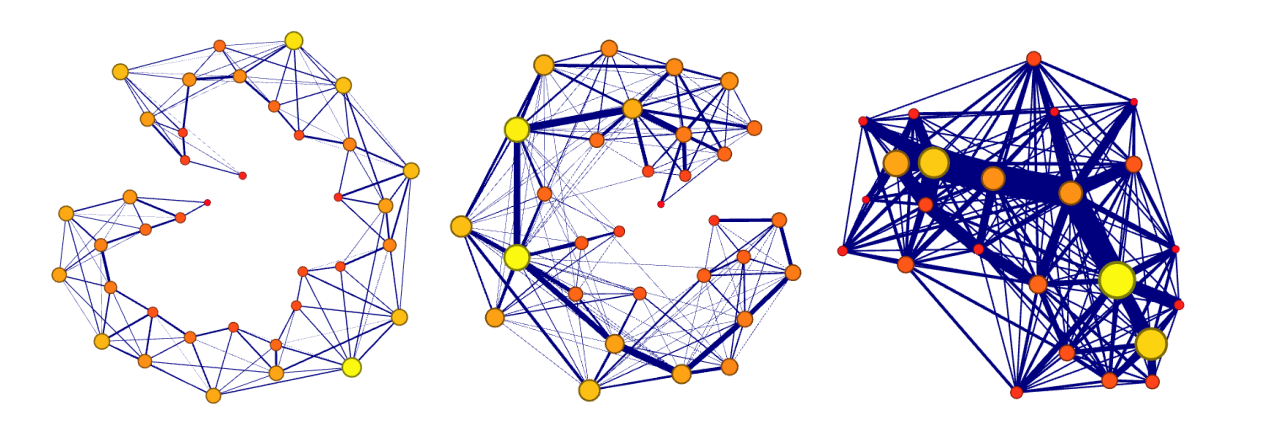
\includegraphics[width=.9\linewidth]{figures/l06/community-structure-and-learning.png}
\vspace*{-1em}
\begin{flushright}
    \footnotesize
    Image Source: \href{https://arxiv.org/pdf/1606.03329}{``Community Structure in Industrial SAT Instances'', Ansotegui et al., AIJ 2019}
\end{flushright}
\end{block}
\end{frame}
    
    
\begin{frame}{Clause Forgetting: Modern Hybrid Approach}
\begin{block}{Manage clauses differently in three tiers}
    \begin{tabularx}{\linewidth}{l|l|X}
        \bf Tier & \bf Strategy & \bf Description\\
        \hline
        \texttt{core} & LBD & Permanently store clauses of LBD $\leq k$ (core-cut value, $3$ in practice)\\
        \texttt{mid-tier} & LRU & Clauses stay here if used in recent conflicts\\
        \texttt{local} & LRU & Keep fixed number of clauses (say $5000$) of highest activity
    \end{tabularx}
\end{block}
\begin{block}{History}
    \begin{itemize}
    \item \texttt{core} and \texttt{local} tier introduced in SWDiA5BY (Chanseok Oh, 2014)
    \item \texttt{mid-tier} introduced in CoMinisatPS (Chanseok Oh, 2015)
    \item \href{https://link.springer.com/chapter/10.1007/978-3-319-24318-4_23}{``Between SAT and UNSAT: The Fundamental Difference in CDCL SAT'' (Chanseok Oh, 2015)}
    \item Note: MapleCOMSPS (2016) is a CoMinisatPS fork
    \end{itemize}
\end{block}
\end{frame}

% \begin{frame}{More on Clause Learning}
% \begin{block}{``Clause Size Reduction with all-UIP Learning''}
%     \begin{itemize}
%     \item Feng \& Bacchus, SAT 2020
%     \item 1-UIP clause has smallest LBD: continue conflict resolution as long as LBD does not increase but clause size decreases
%     \item SAT Competition 2020: \texttt{CaDiCaL AllUIP} (won planning track)
%     \end{itemize}
% \end{block}
% \end{frame}

\graphicspath{ {satvizpdf/} }

\begin{frame}{Visualized Instance: Aprove (Termination Analysis, SAT)}{
    \only<1>{initial layout, recently active variables after 1000 conflicts}
    \only<2>{initial layout, recently active variables after 1690 conflicts}
    \only<3>{initial layout, recently active variables after 3090 conflicts}
    \only<4>{initial layout, recently active variables after 5000 conflicts}
    \only<5>{relayout after 6000 conflicts}
    \only<6>{core after 52500 conflicts}
}
\centering
\vspace*{-1em}
\only<1>{
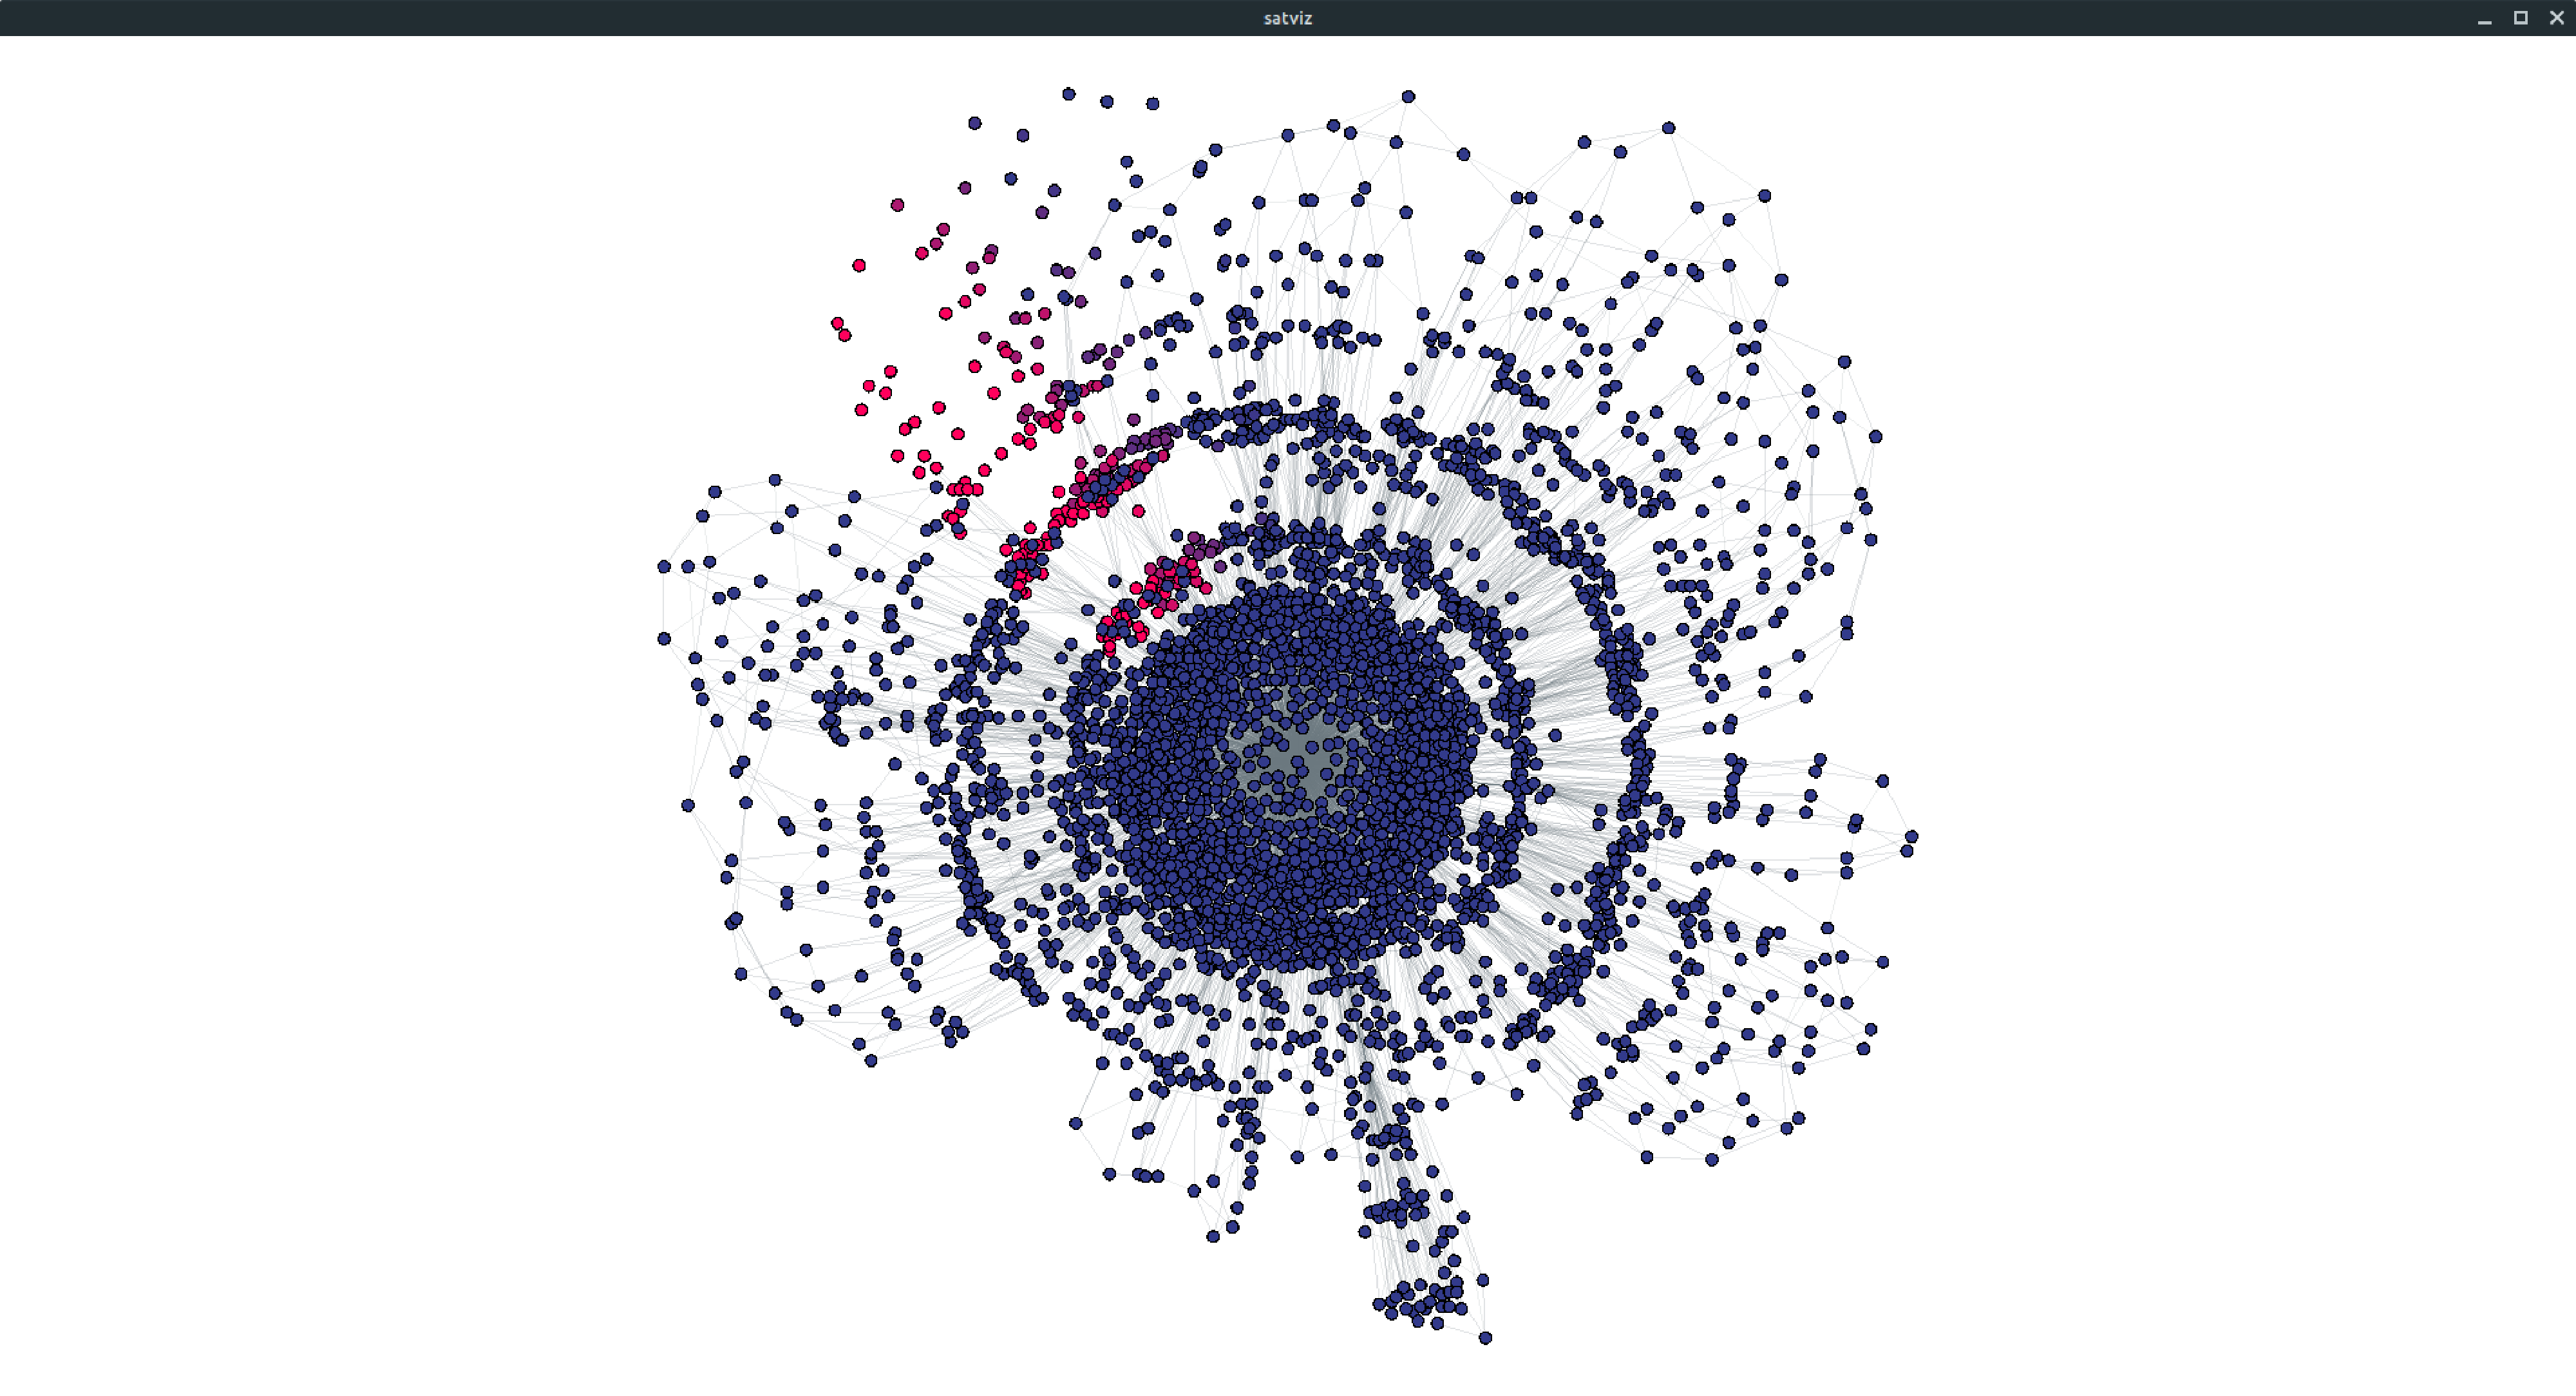
\includegraphics[width=0.9\textwidth, trim={100 0 100 100}, clip]{satviz-aprove-1000}
}
\only<2>{
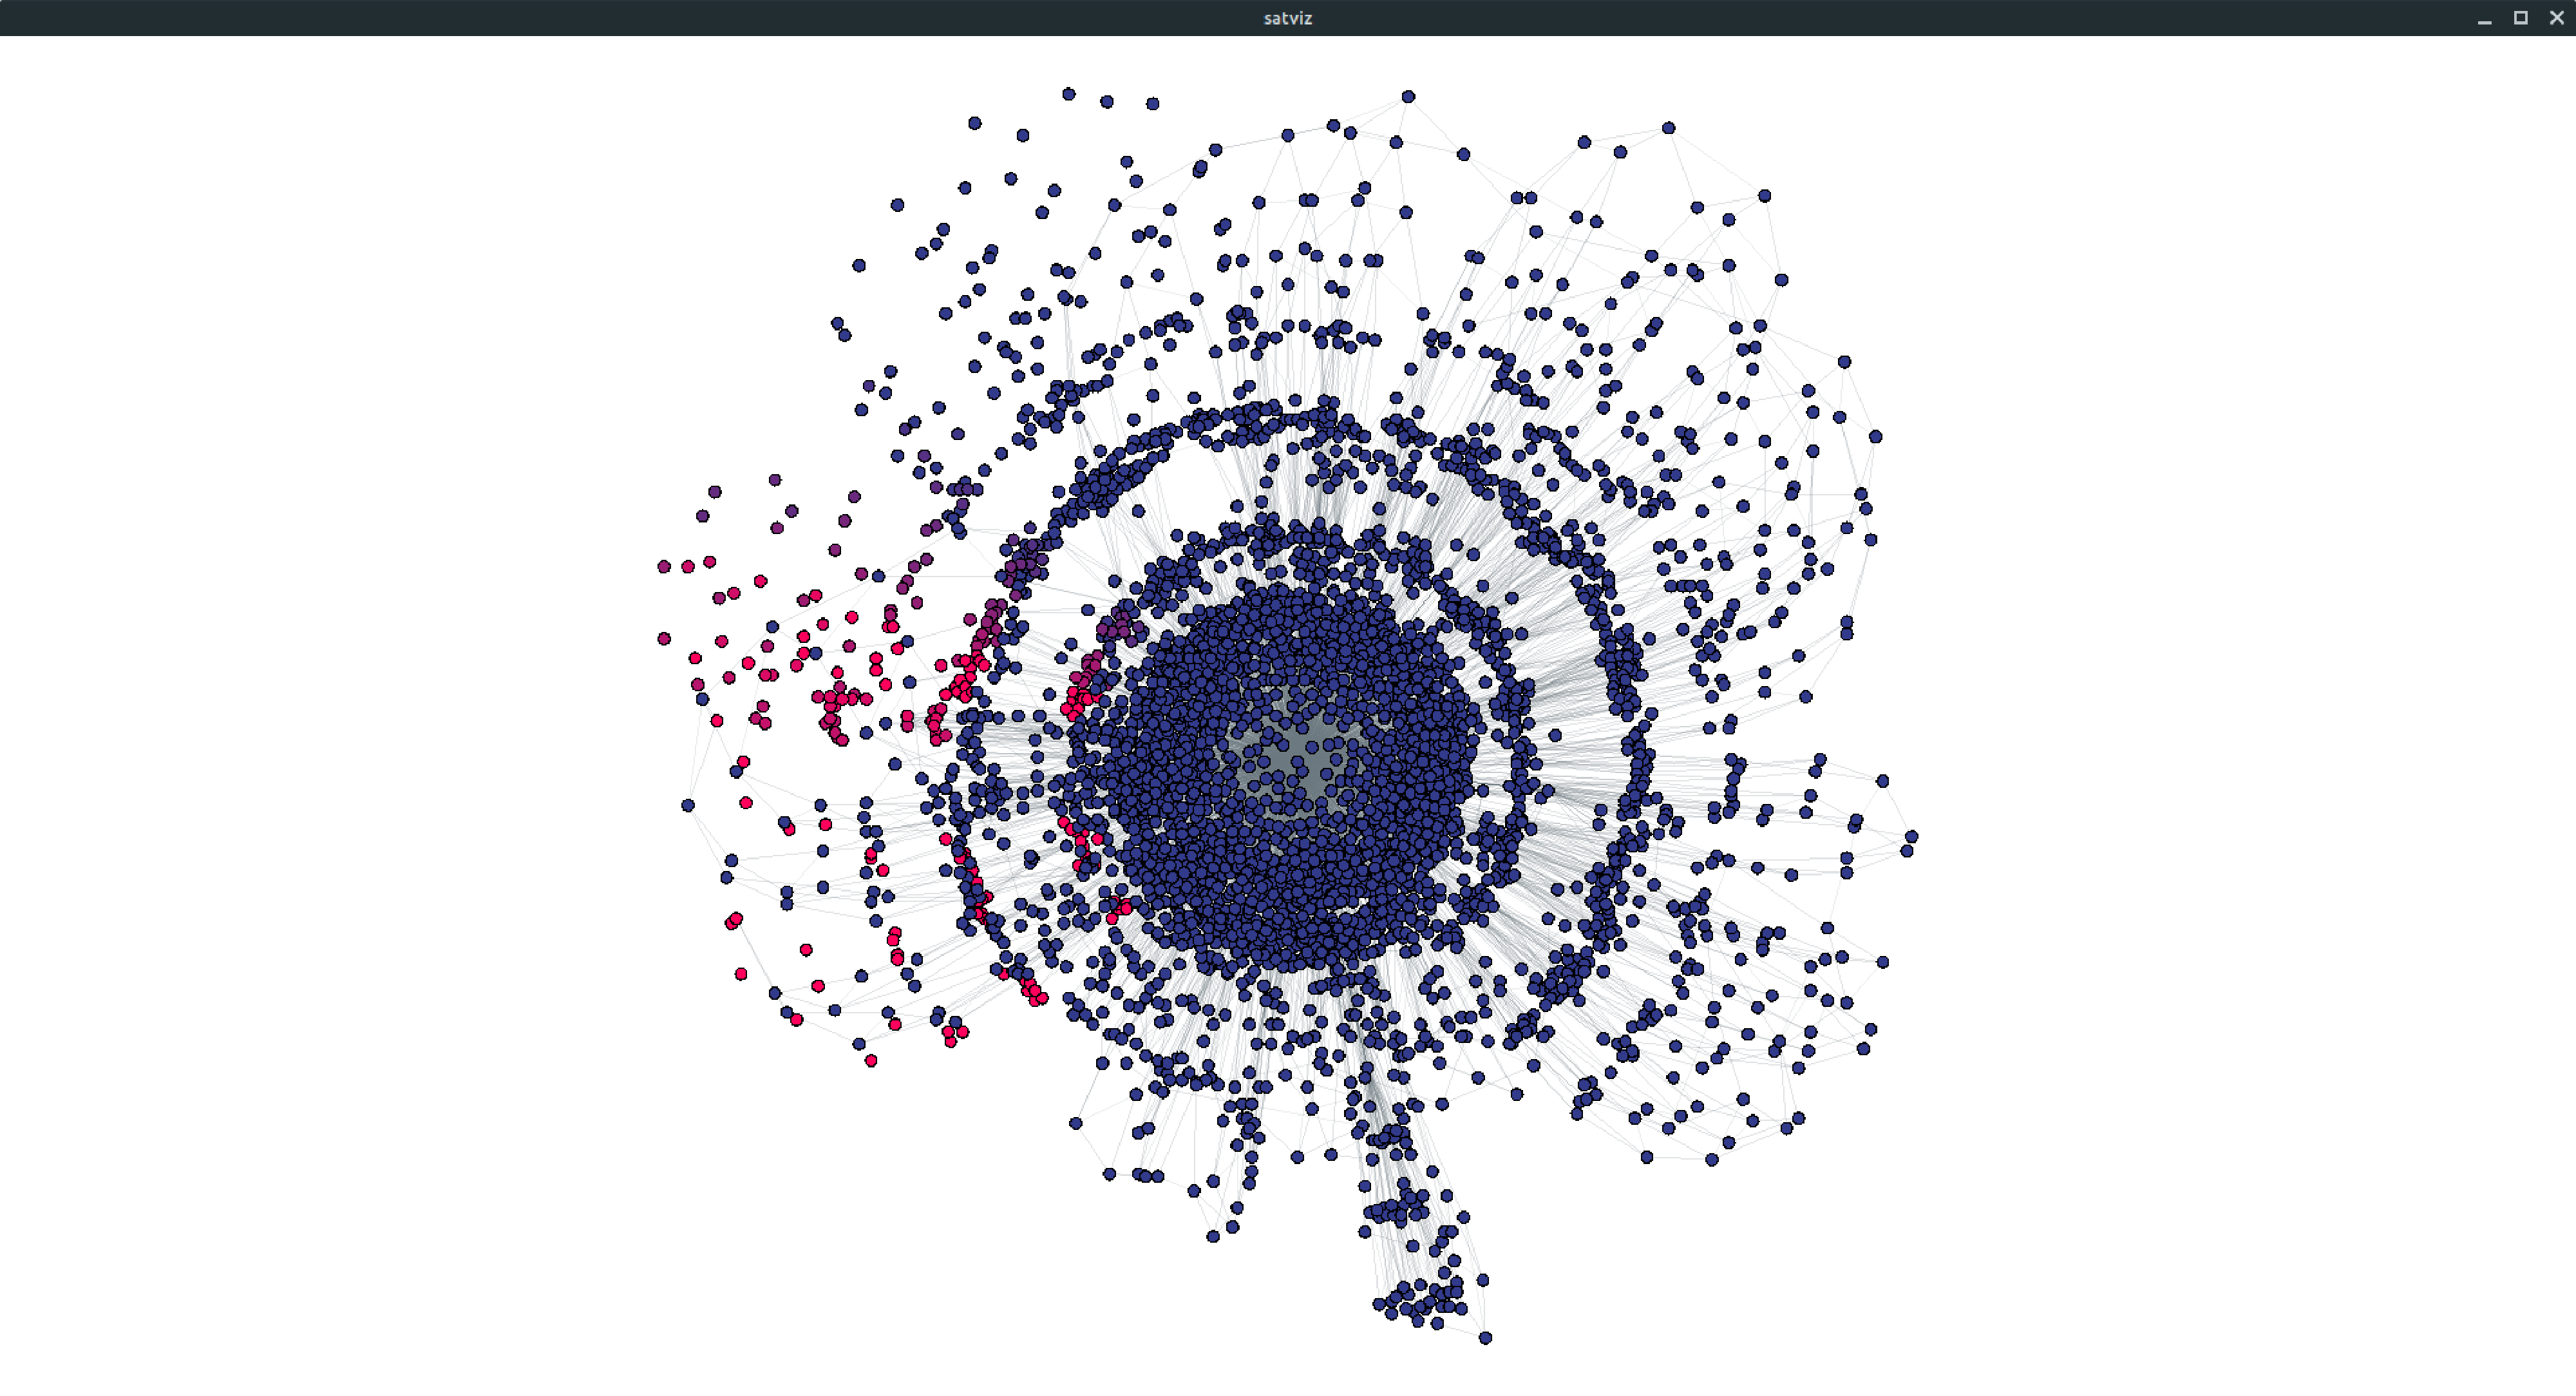
\includegraphics[width=0.9\textwidth, trim={100 0 100 100}, clip]{satviz-aprove-1690}
}
\only<3>{
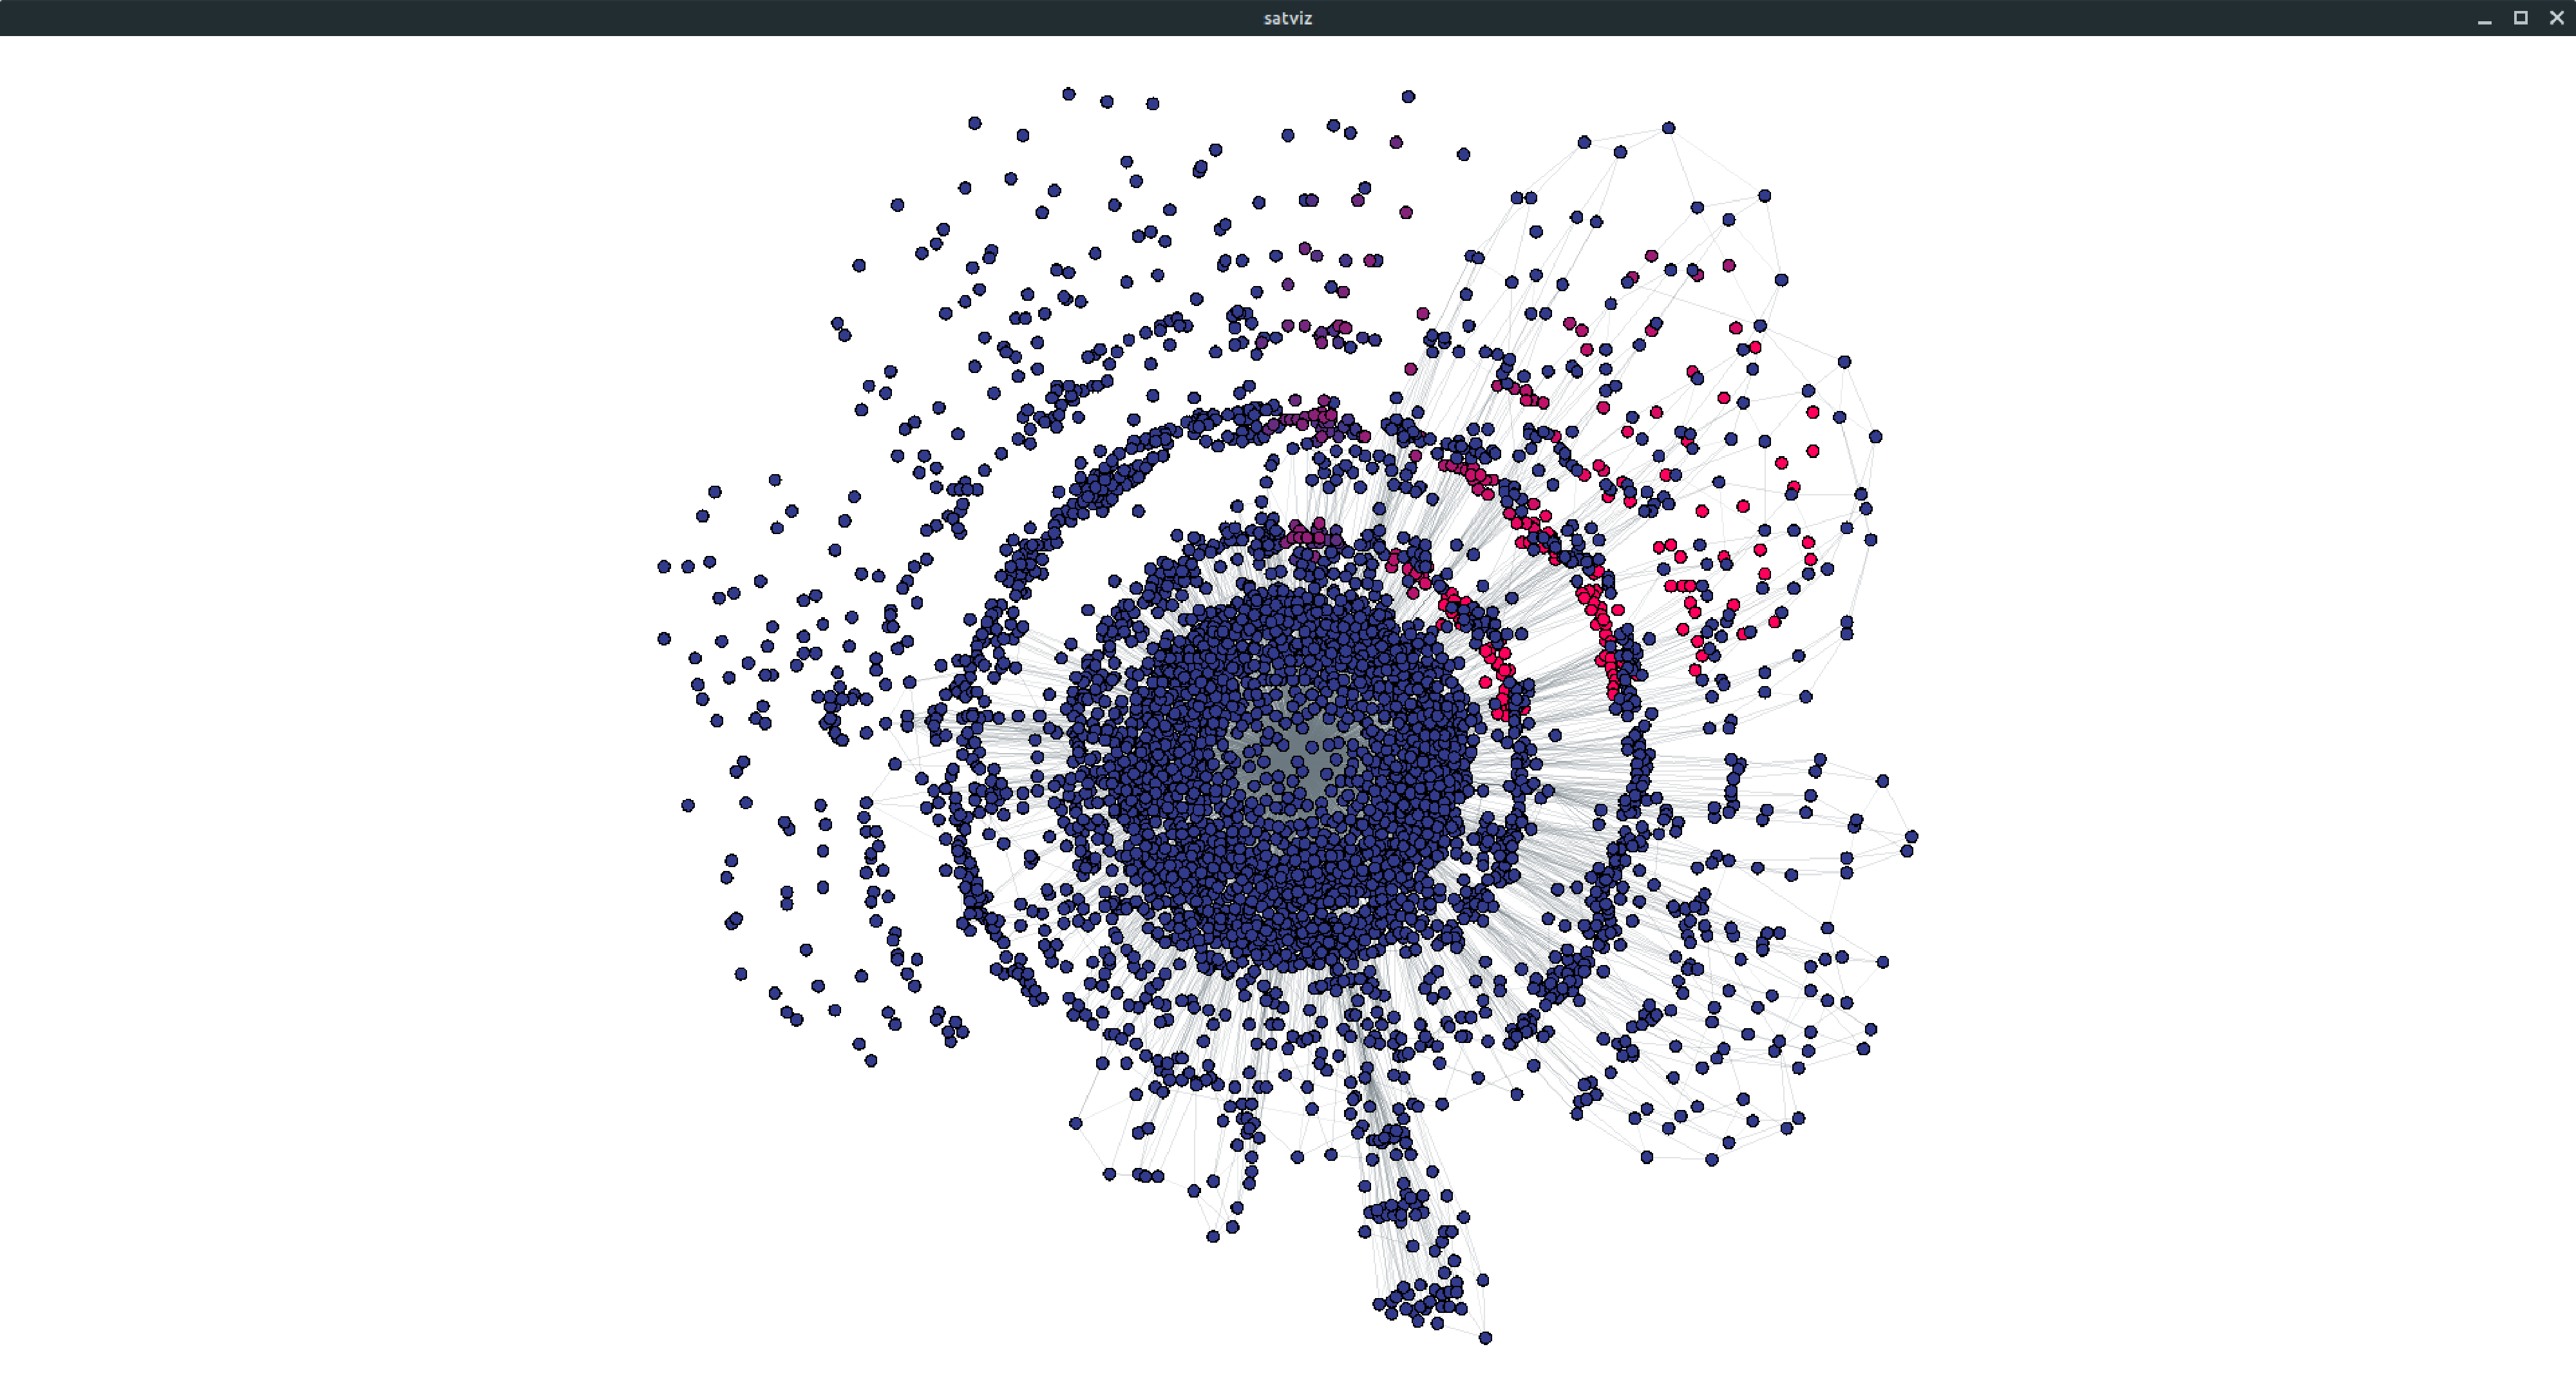
\includegraphics[width=0.9\textwidth, trim={100 0 100 100}, clip]{satviz-aprove-3090}
}
\only<4>{
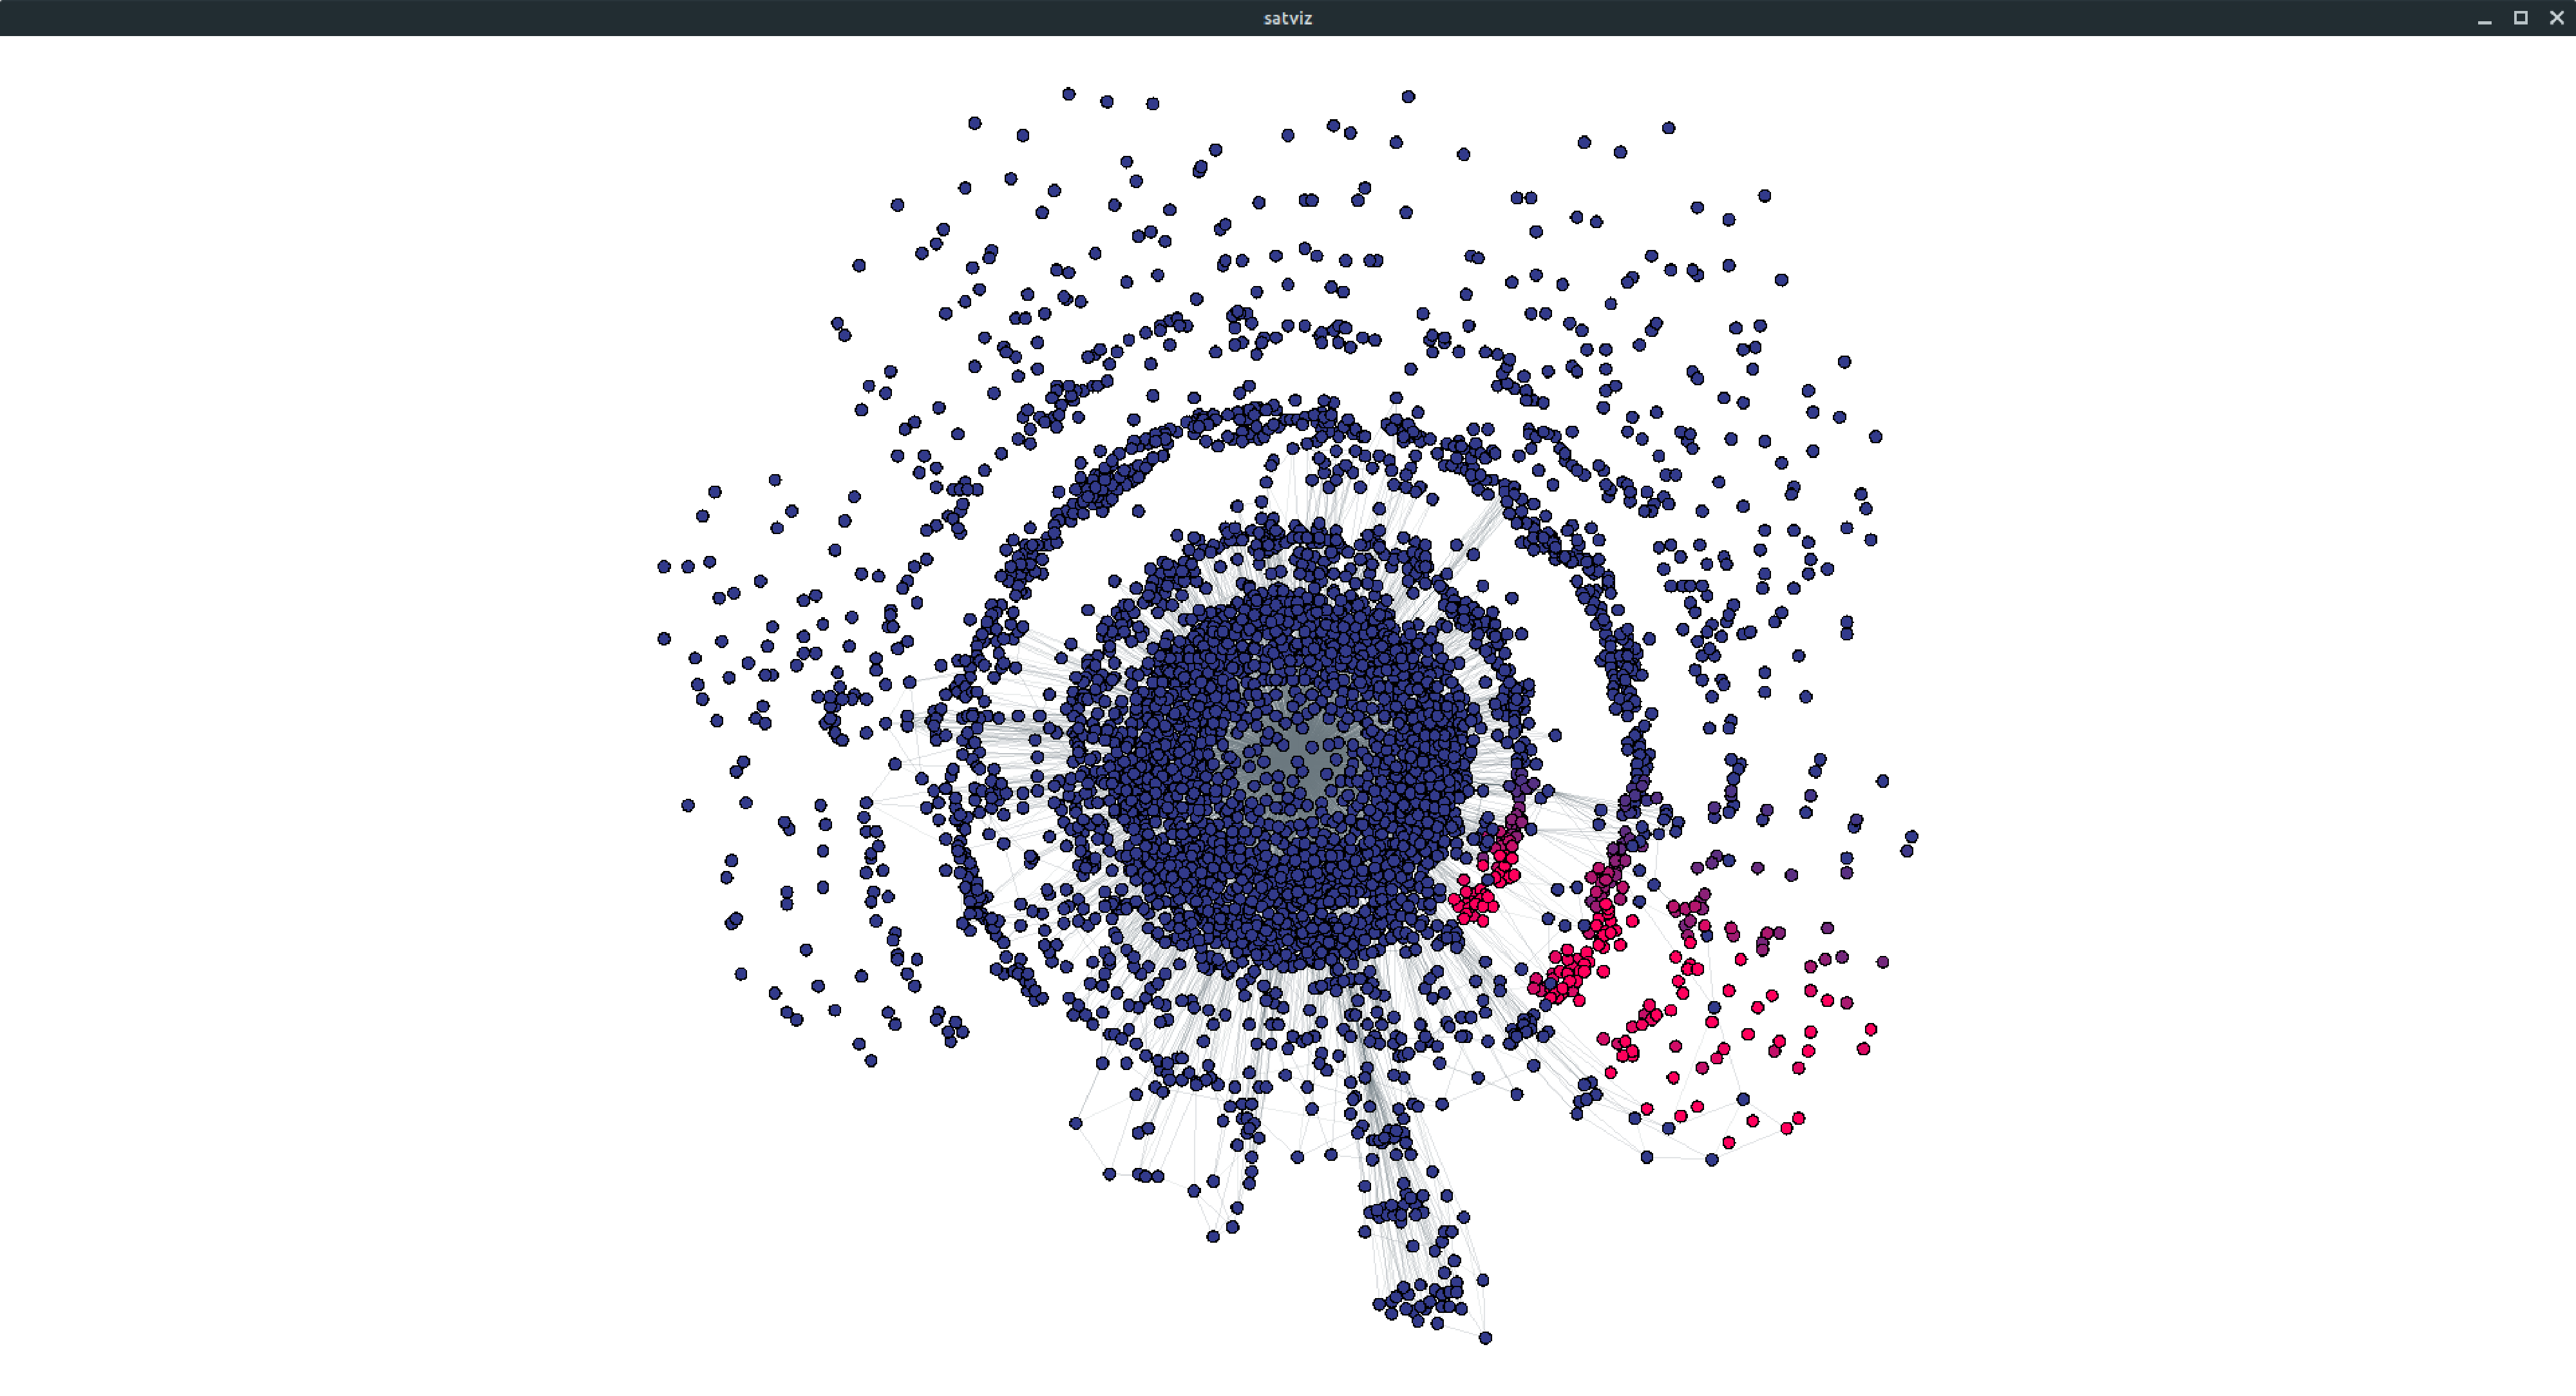
\includegraphics[width=0.9\textwidth, trim={100 0 100 100}, clip]{satviz-aprove-5000}
}
\only<5>{
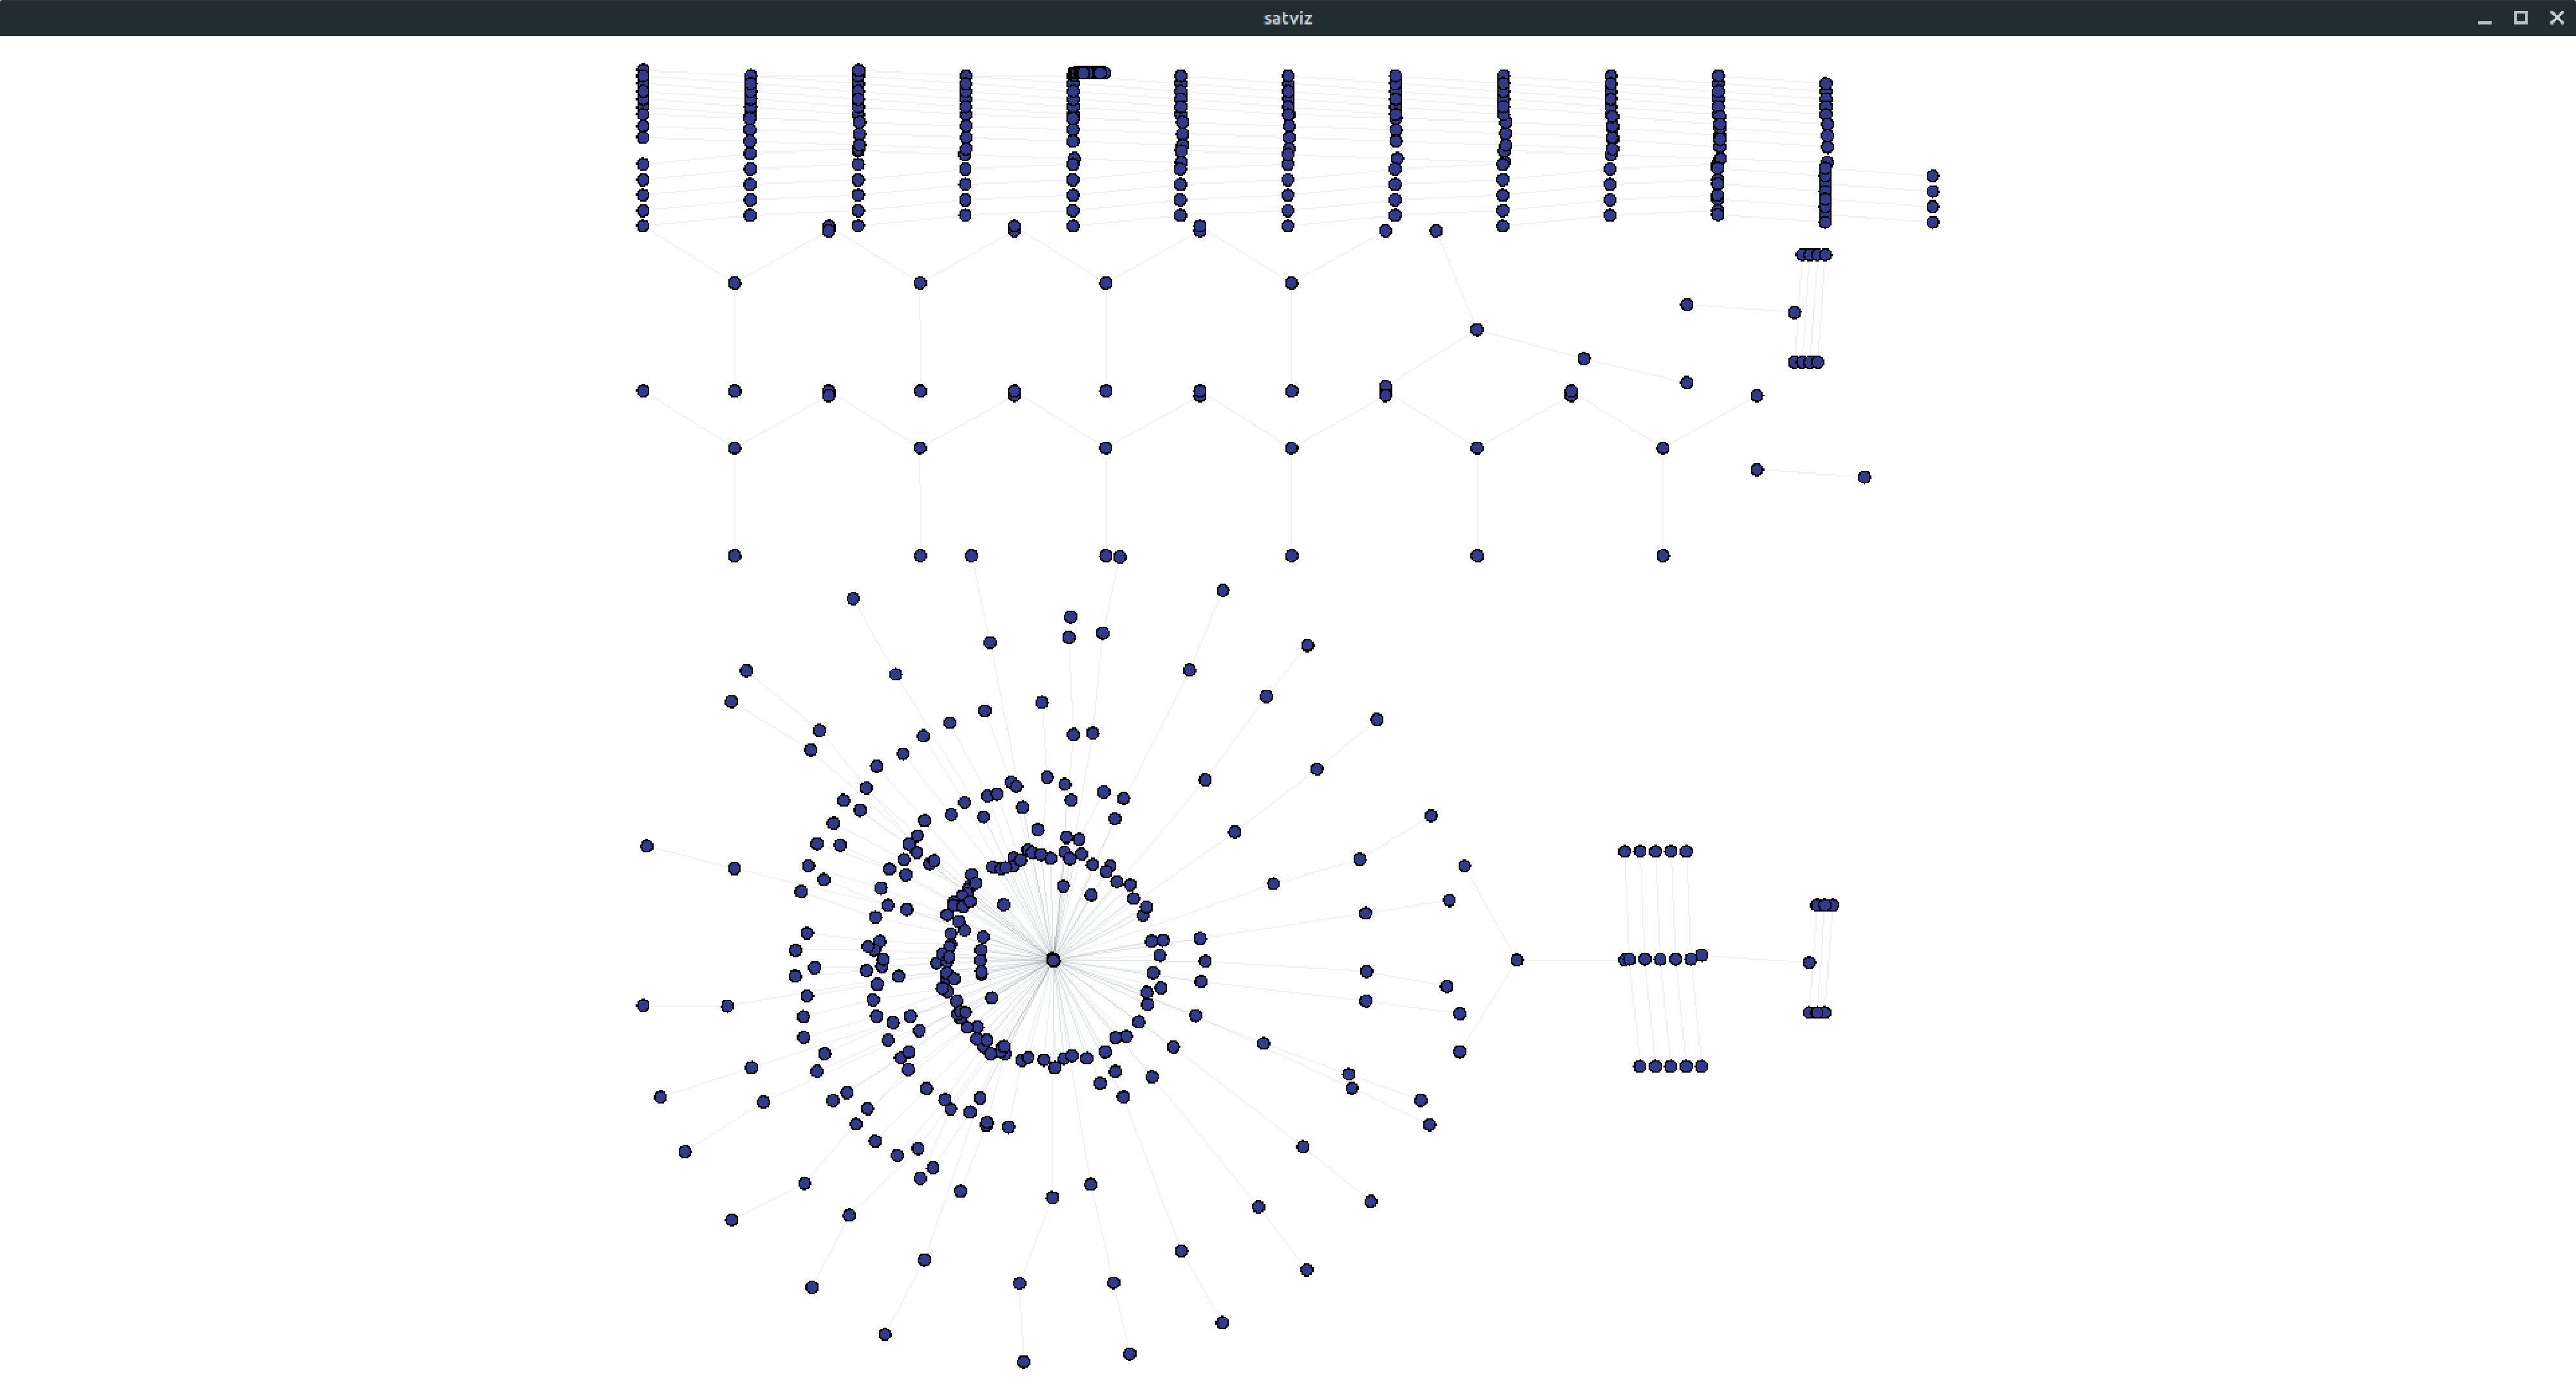
\includegraphics[width=0.9\textwidth, trim={100 0 100 100}, clip]{satviz-aprove-6000-relayout}
}
\only<6>{
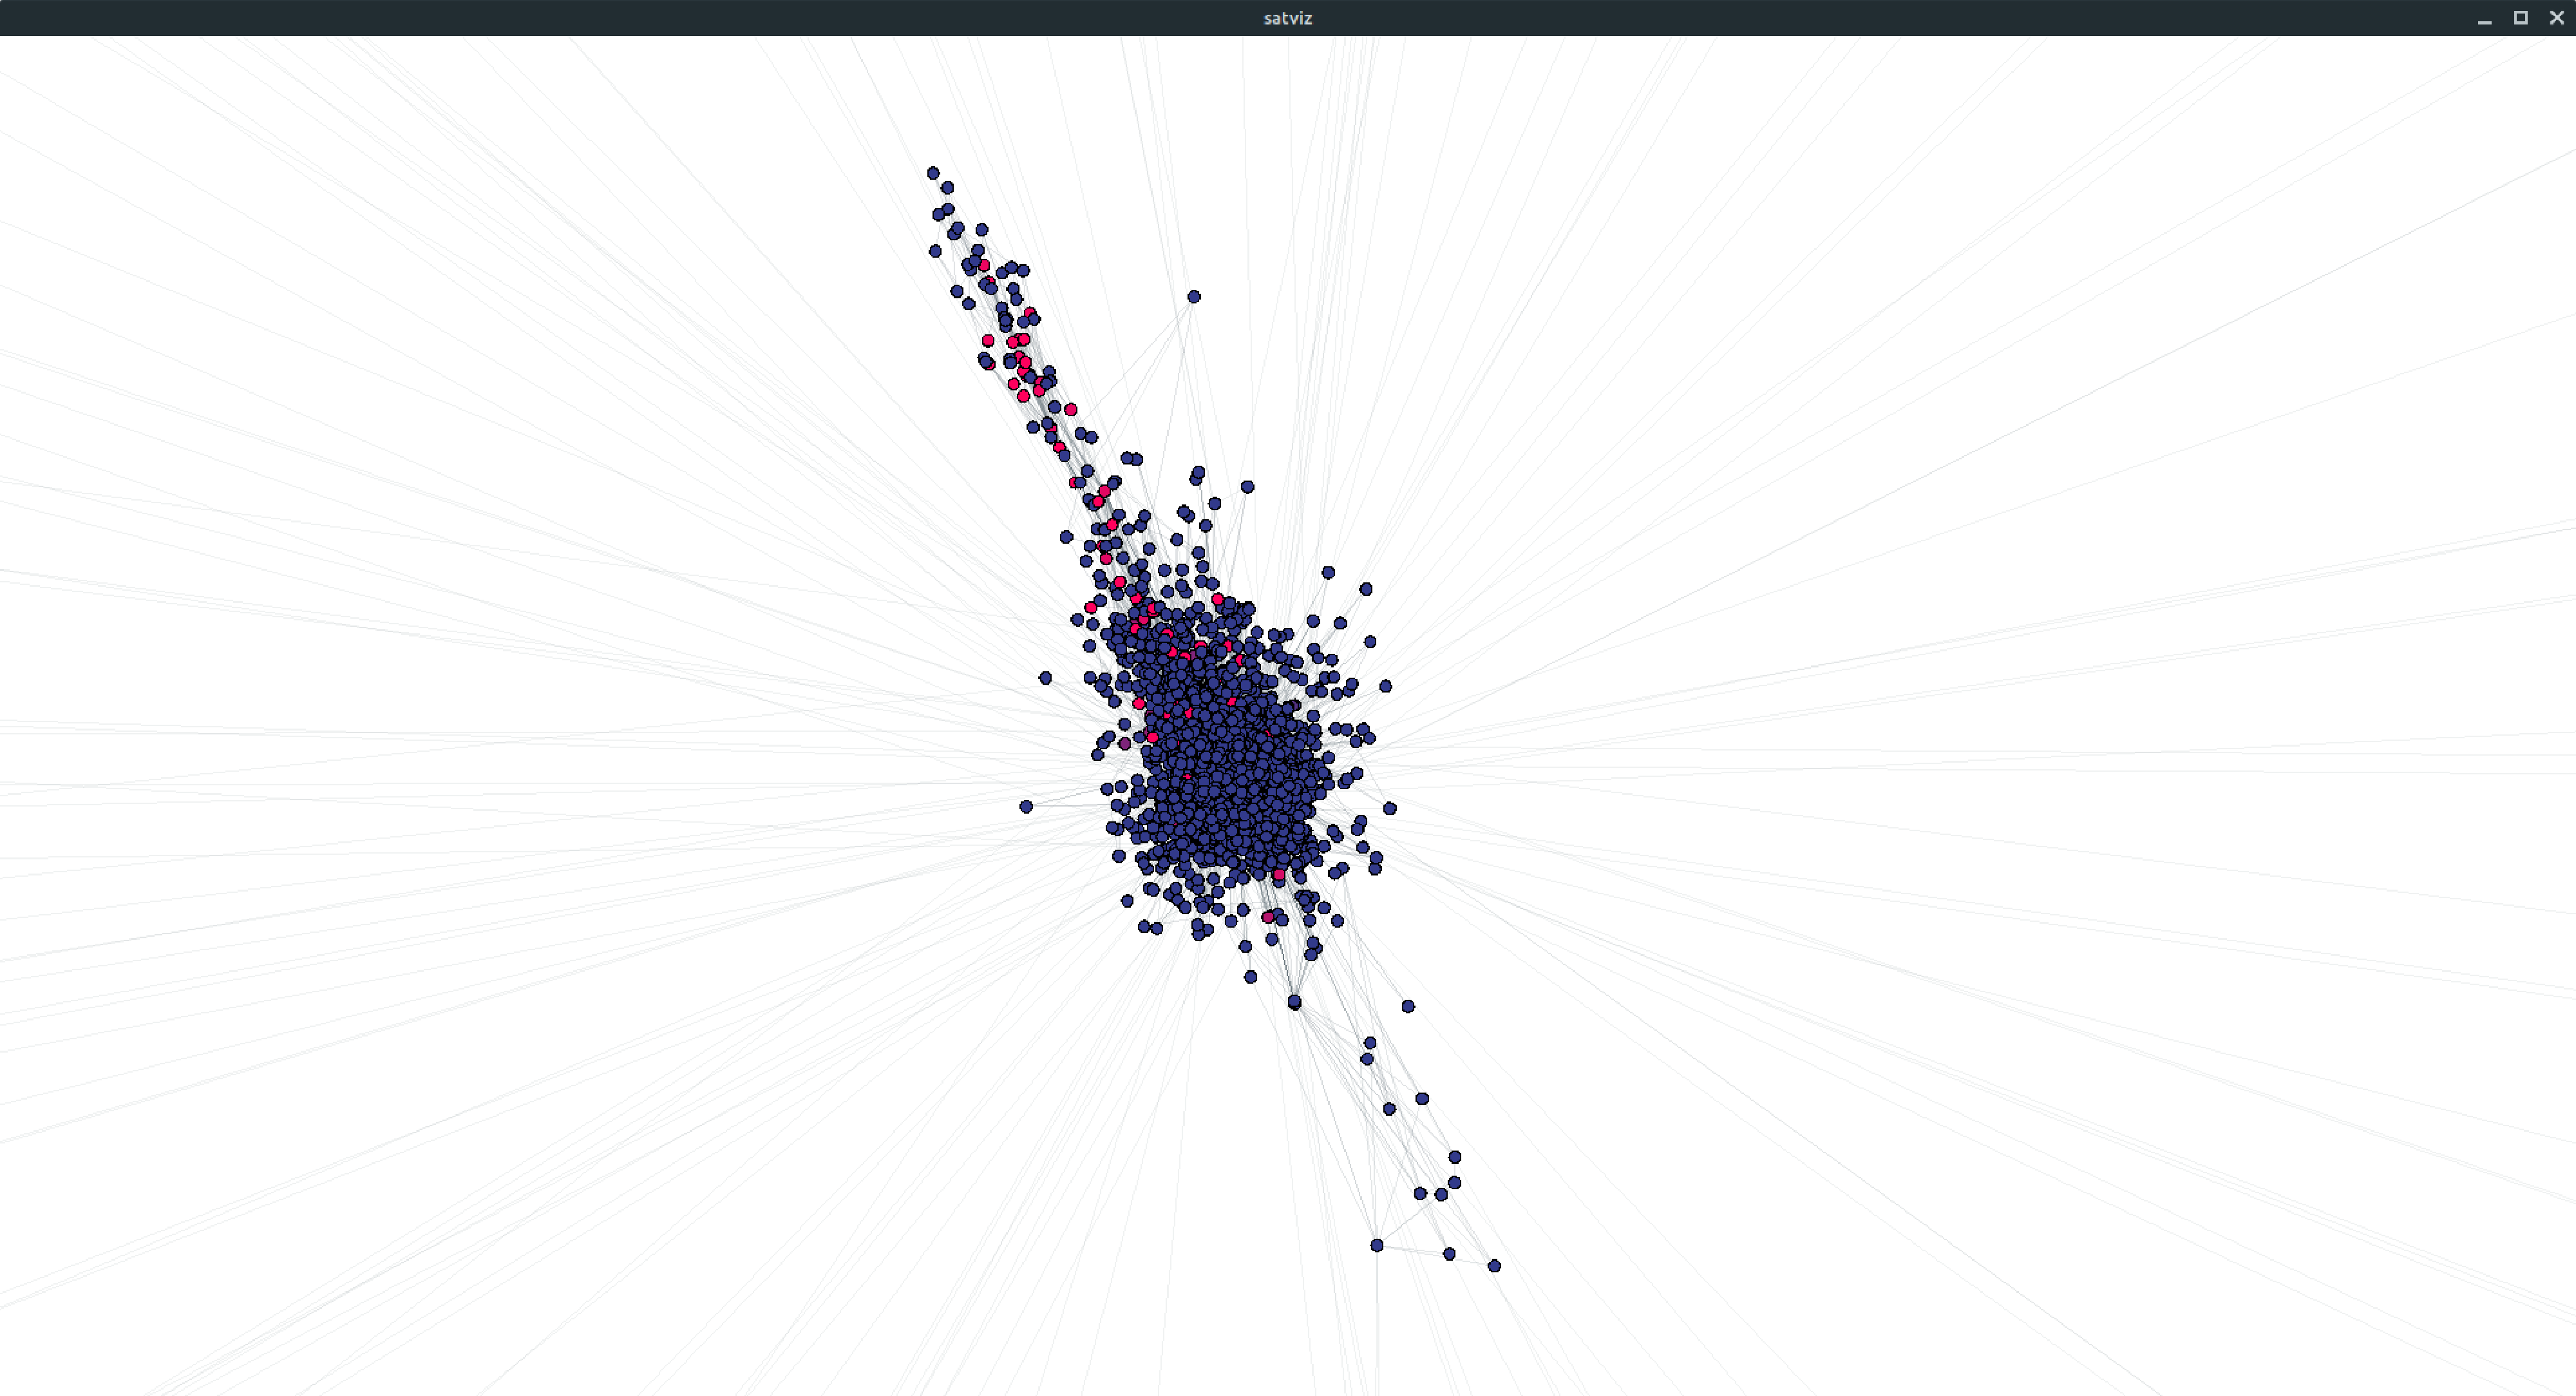
\includegraphics[width=0.9\textwidth, trim={100 0 100 100}, clip]{satviz-aprove-52500-zoom}
}
\end{frame}

\begin{frame}{Visualized Instance: Newton SMT (SV Competition, SAT)}{
    \only<1>{initial layout}
    \only<2>{after 10000 conflicts}
    \only<3>{after 1000000 conflicts}
    \only<4>{after 3000000 conflicts}
    \only<5>{core, after 3500000 conflicts, almost solved}
}
\centering
\vspace*{-2em}
\only<1>{
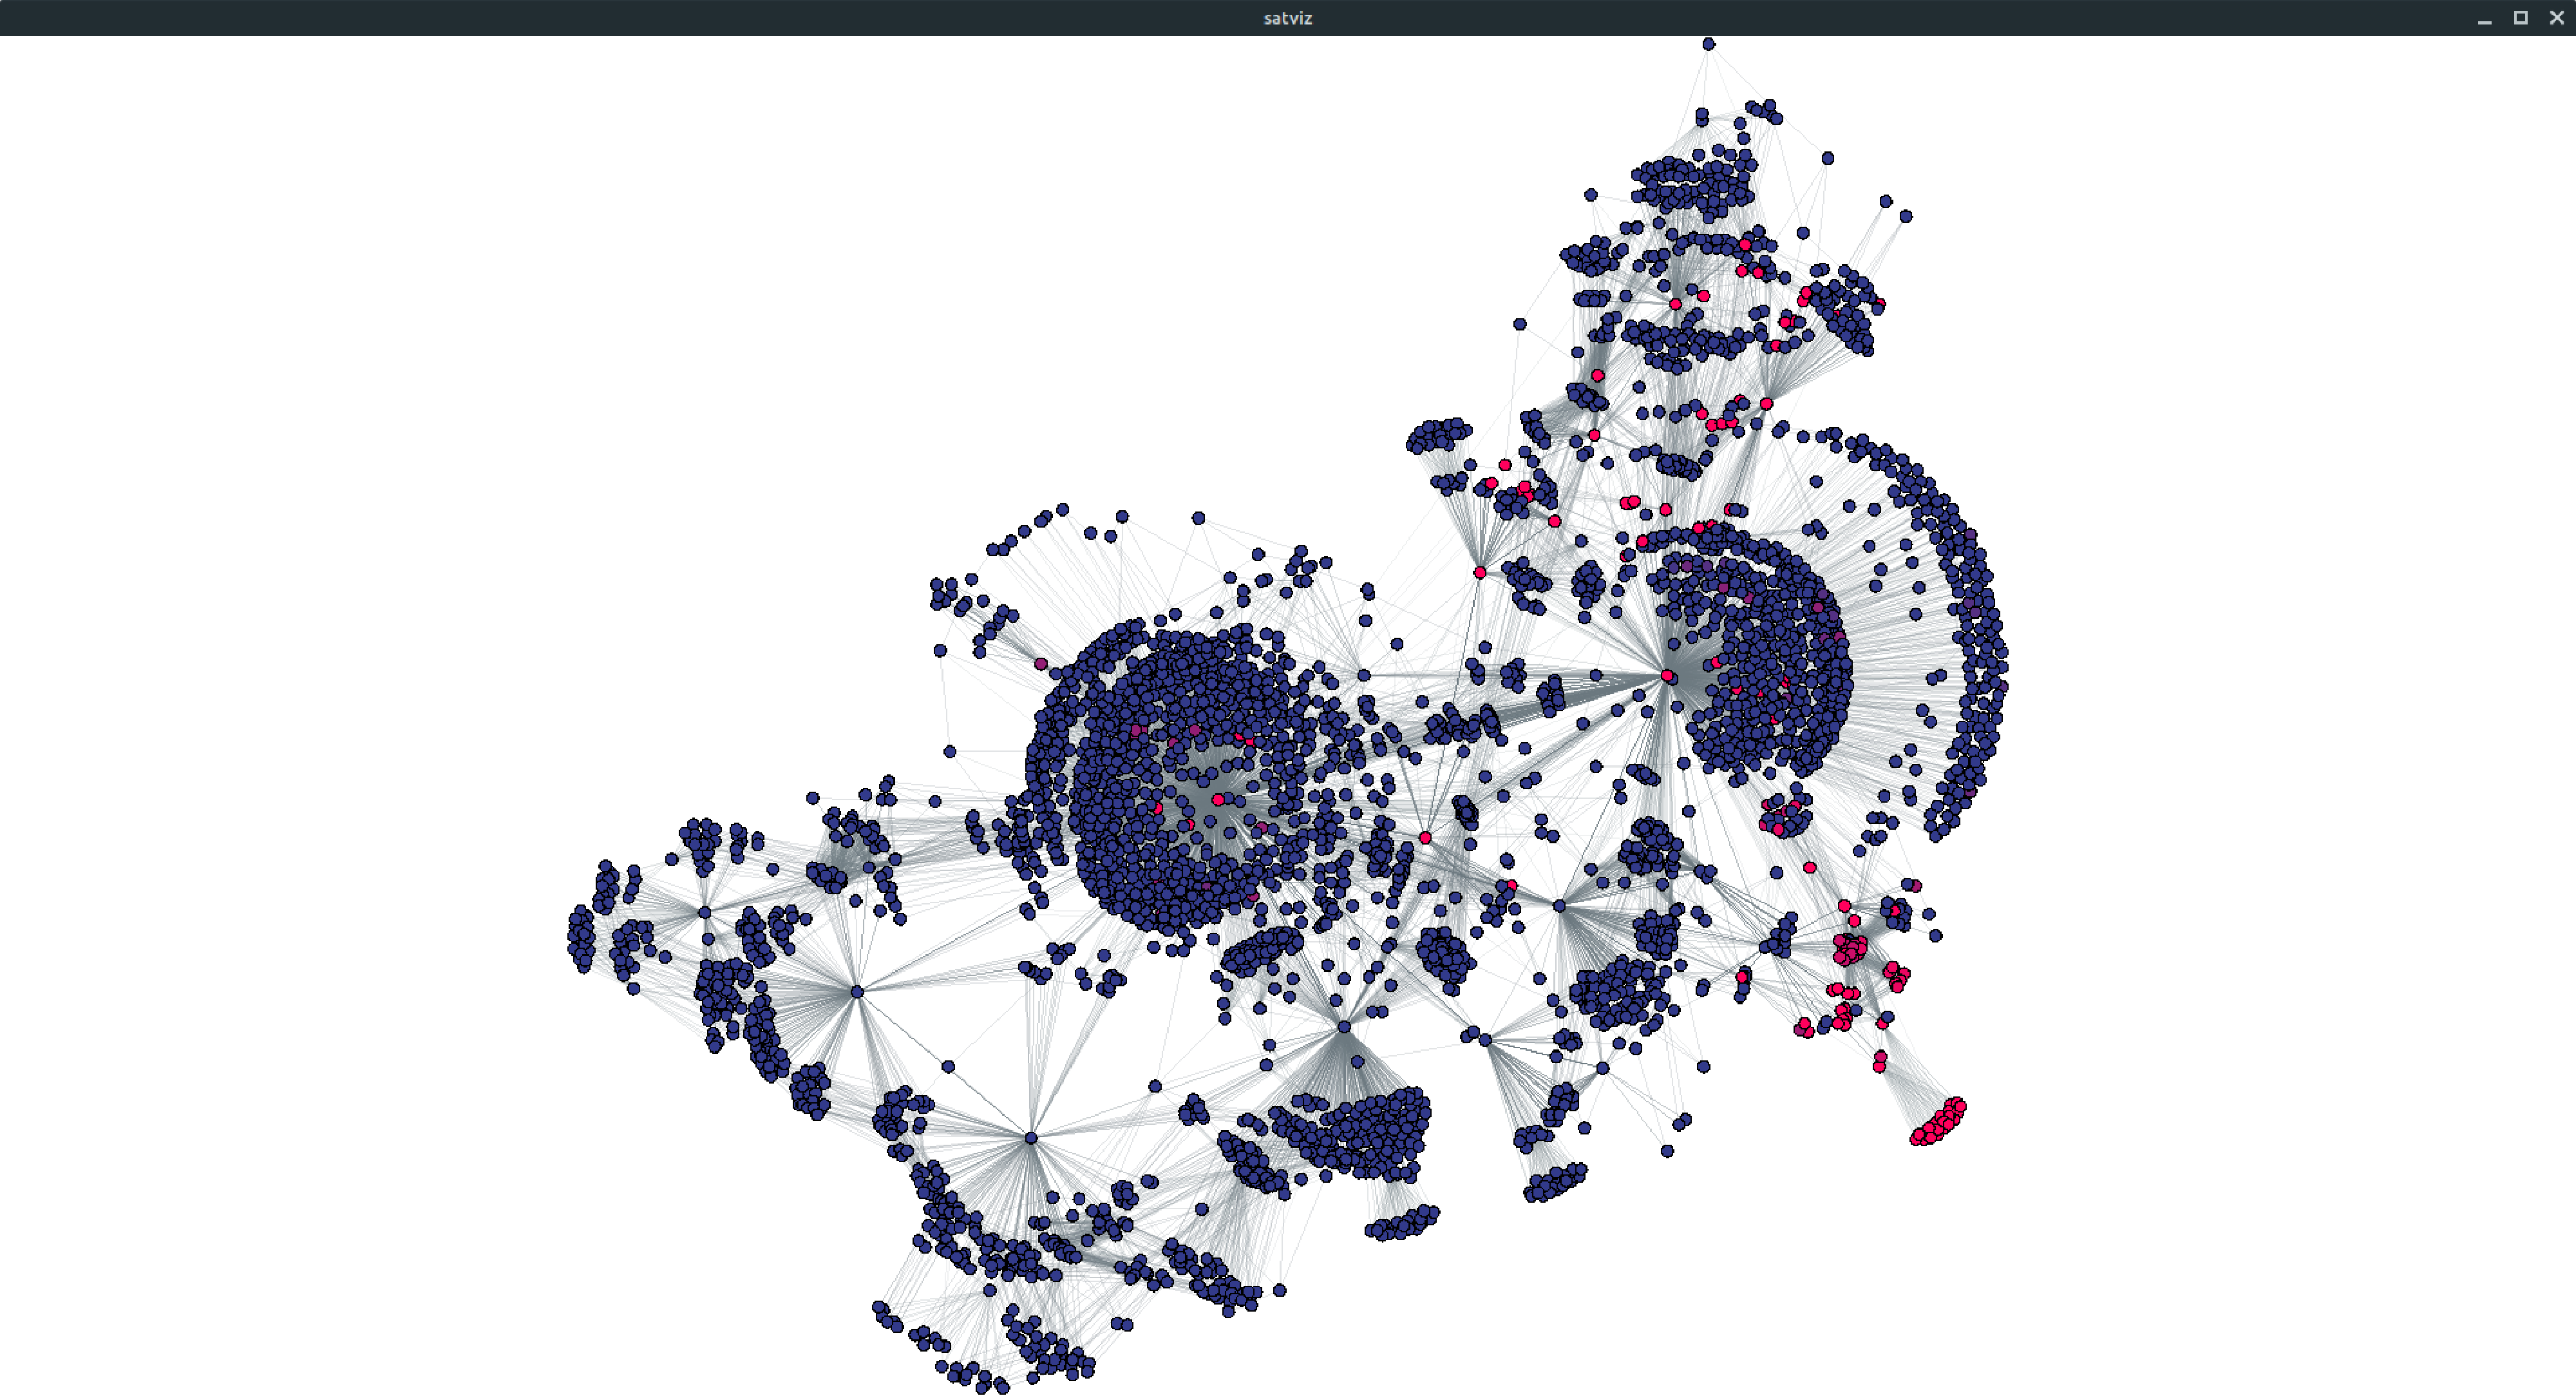
\includegraphics[width=0.9\textwidth, trim={100 0 100 100}, clip]{newton-smt-5200}
}
\only<2>{
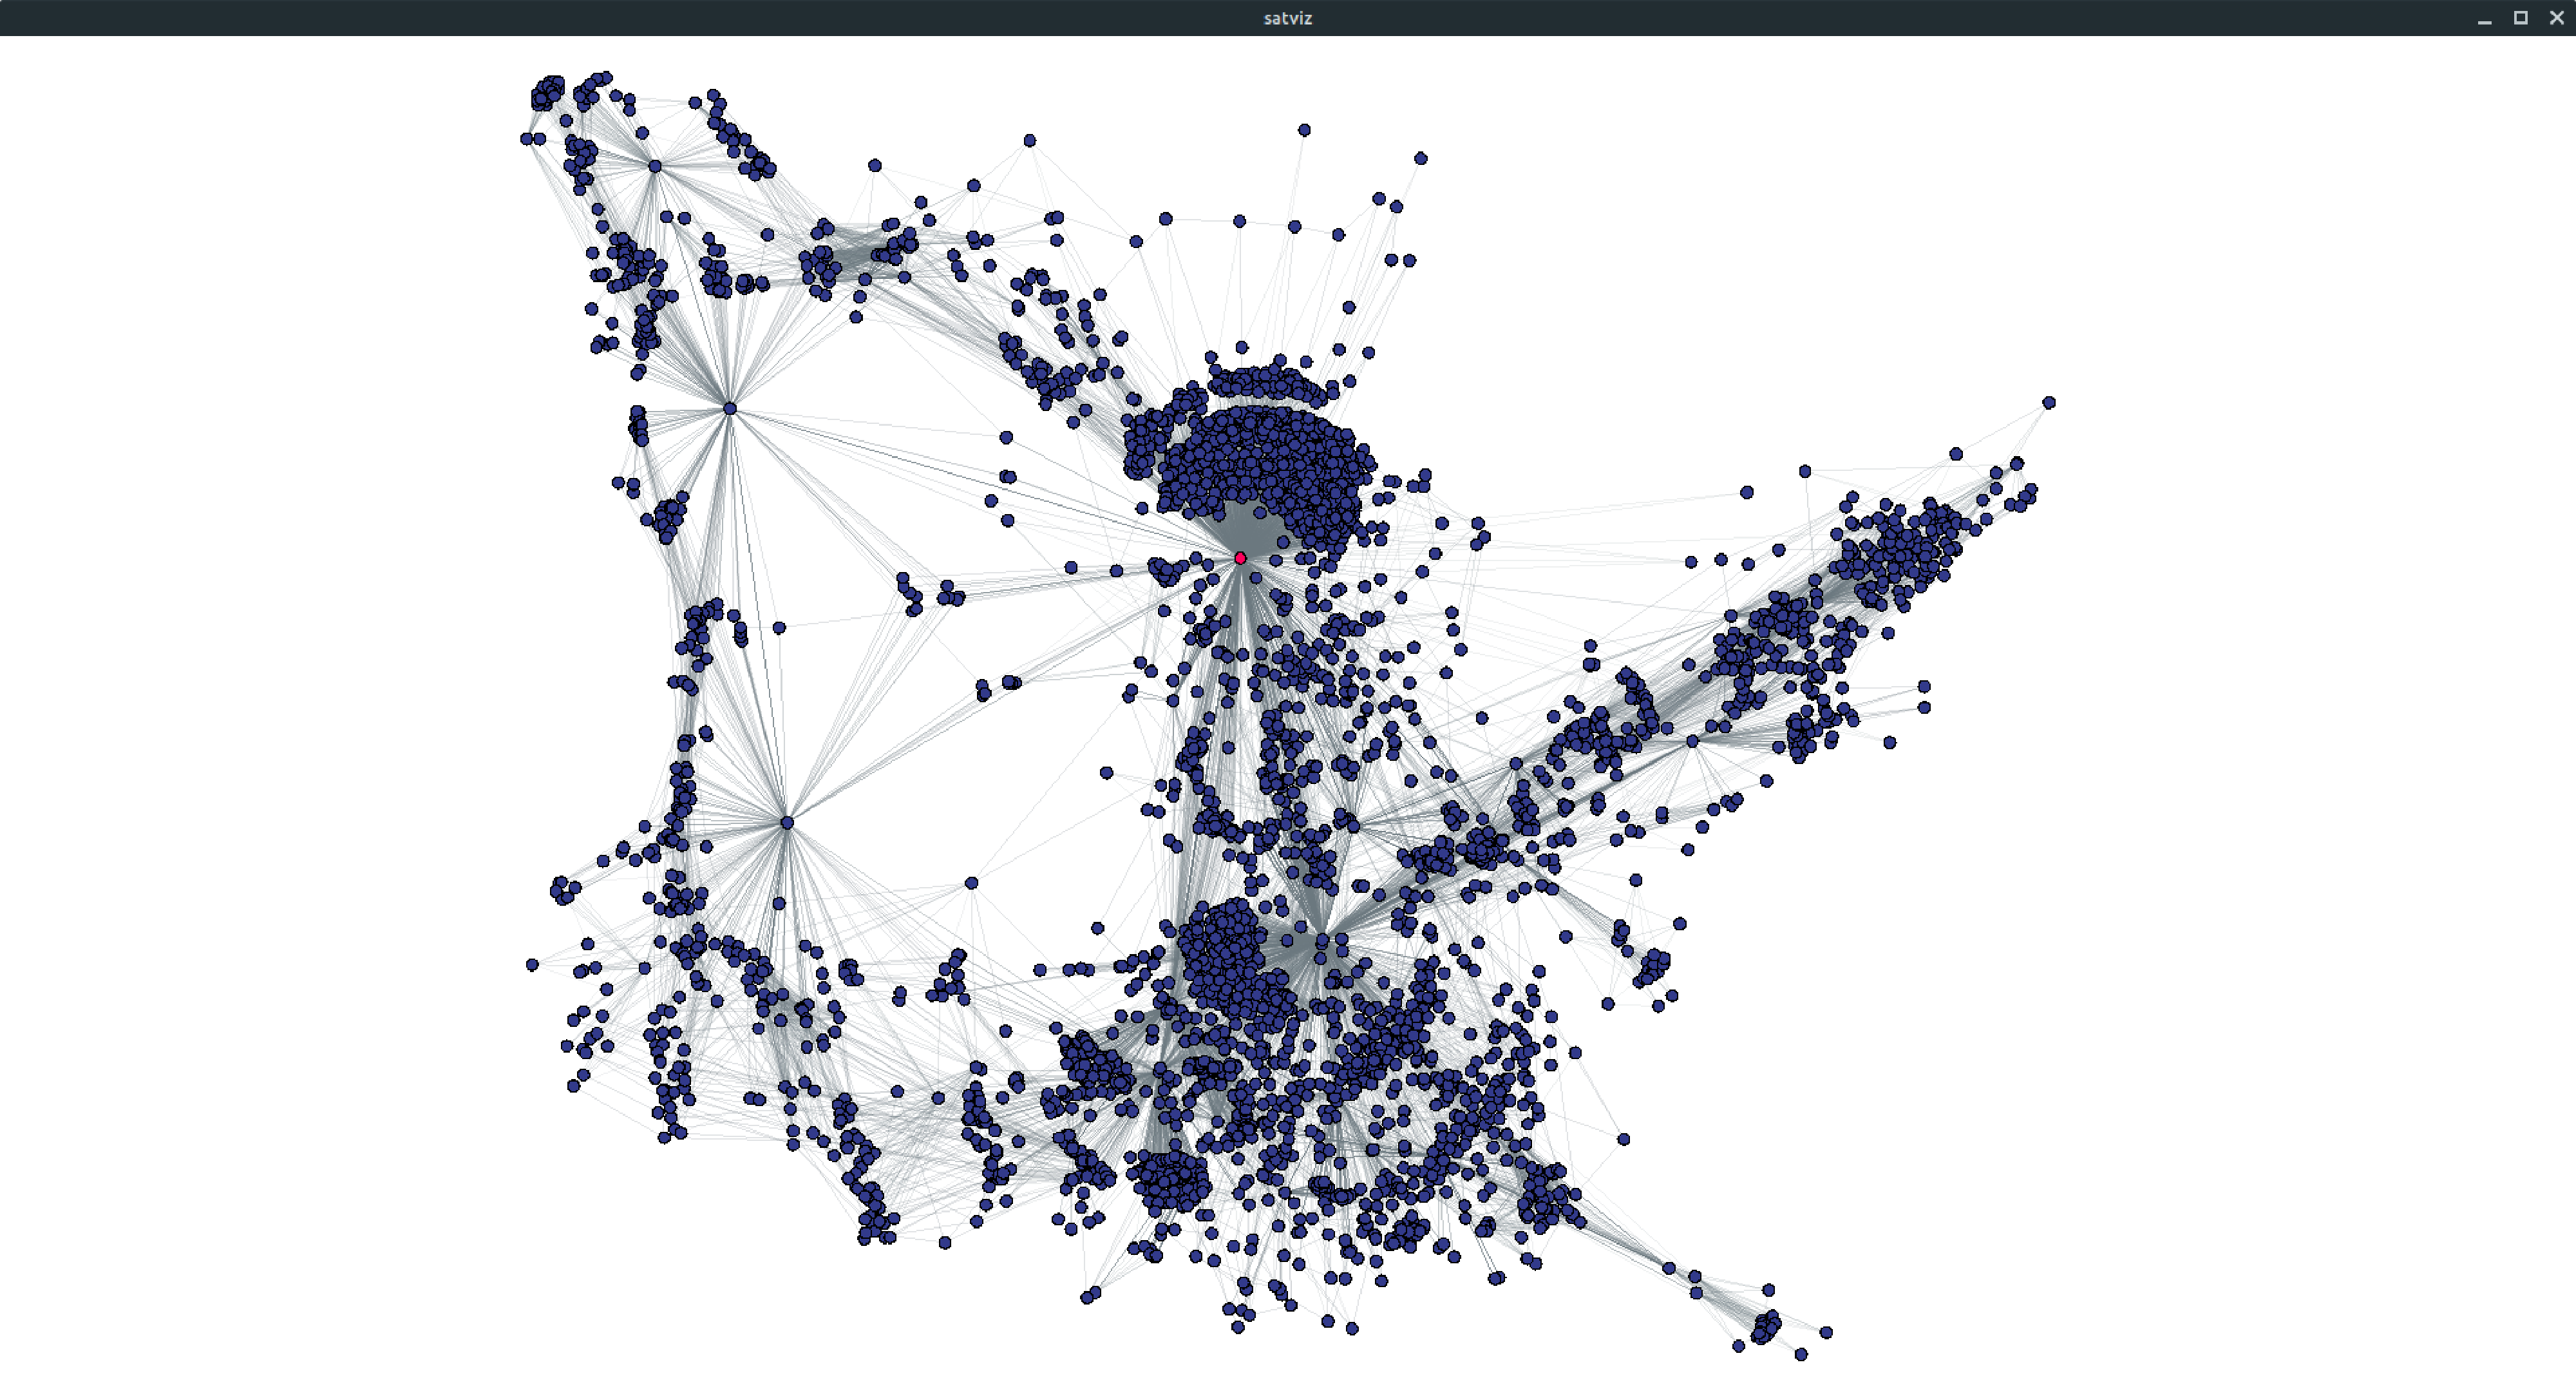
\includegraphics[width=0.9\textwidth, trim={100 0 100 100}, clip]{newton-smt-10000}
}
\only<3>{
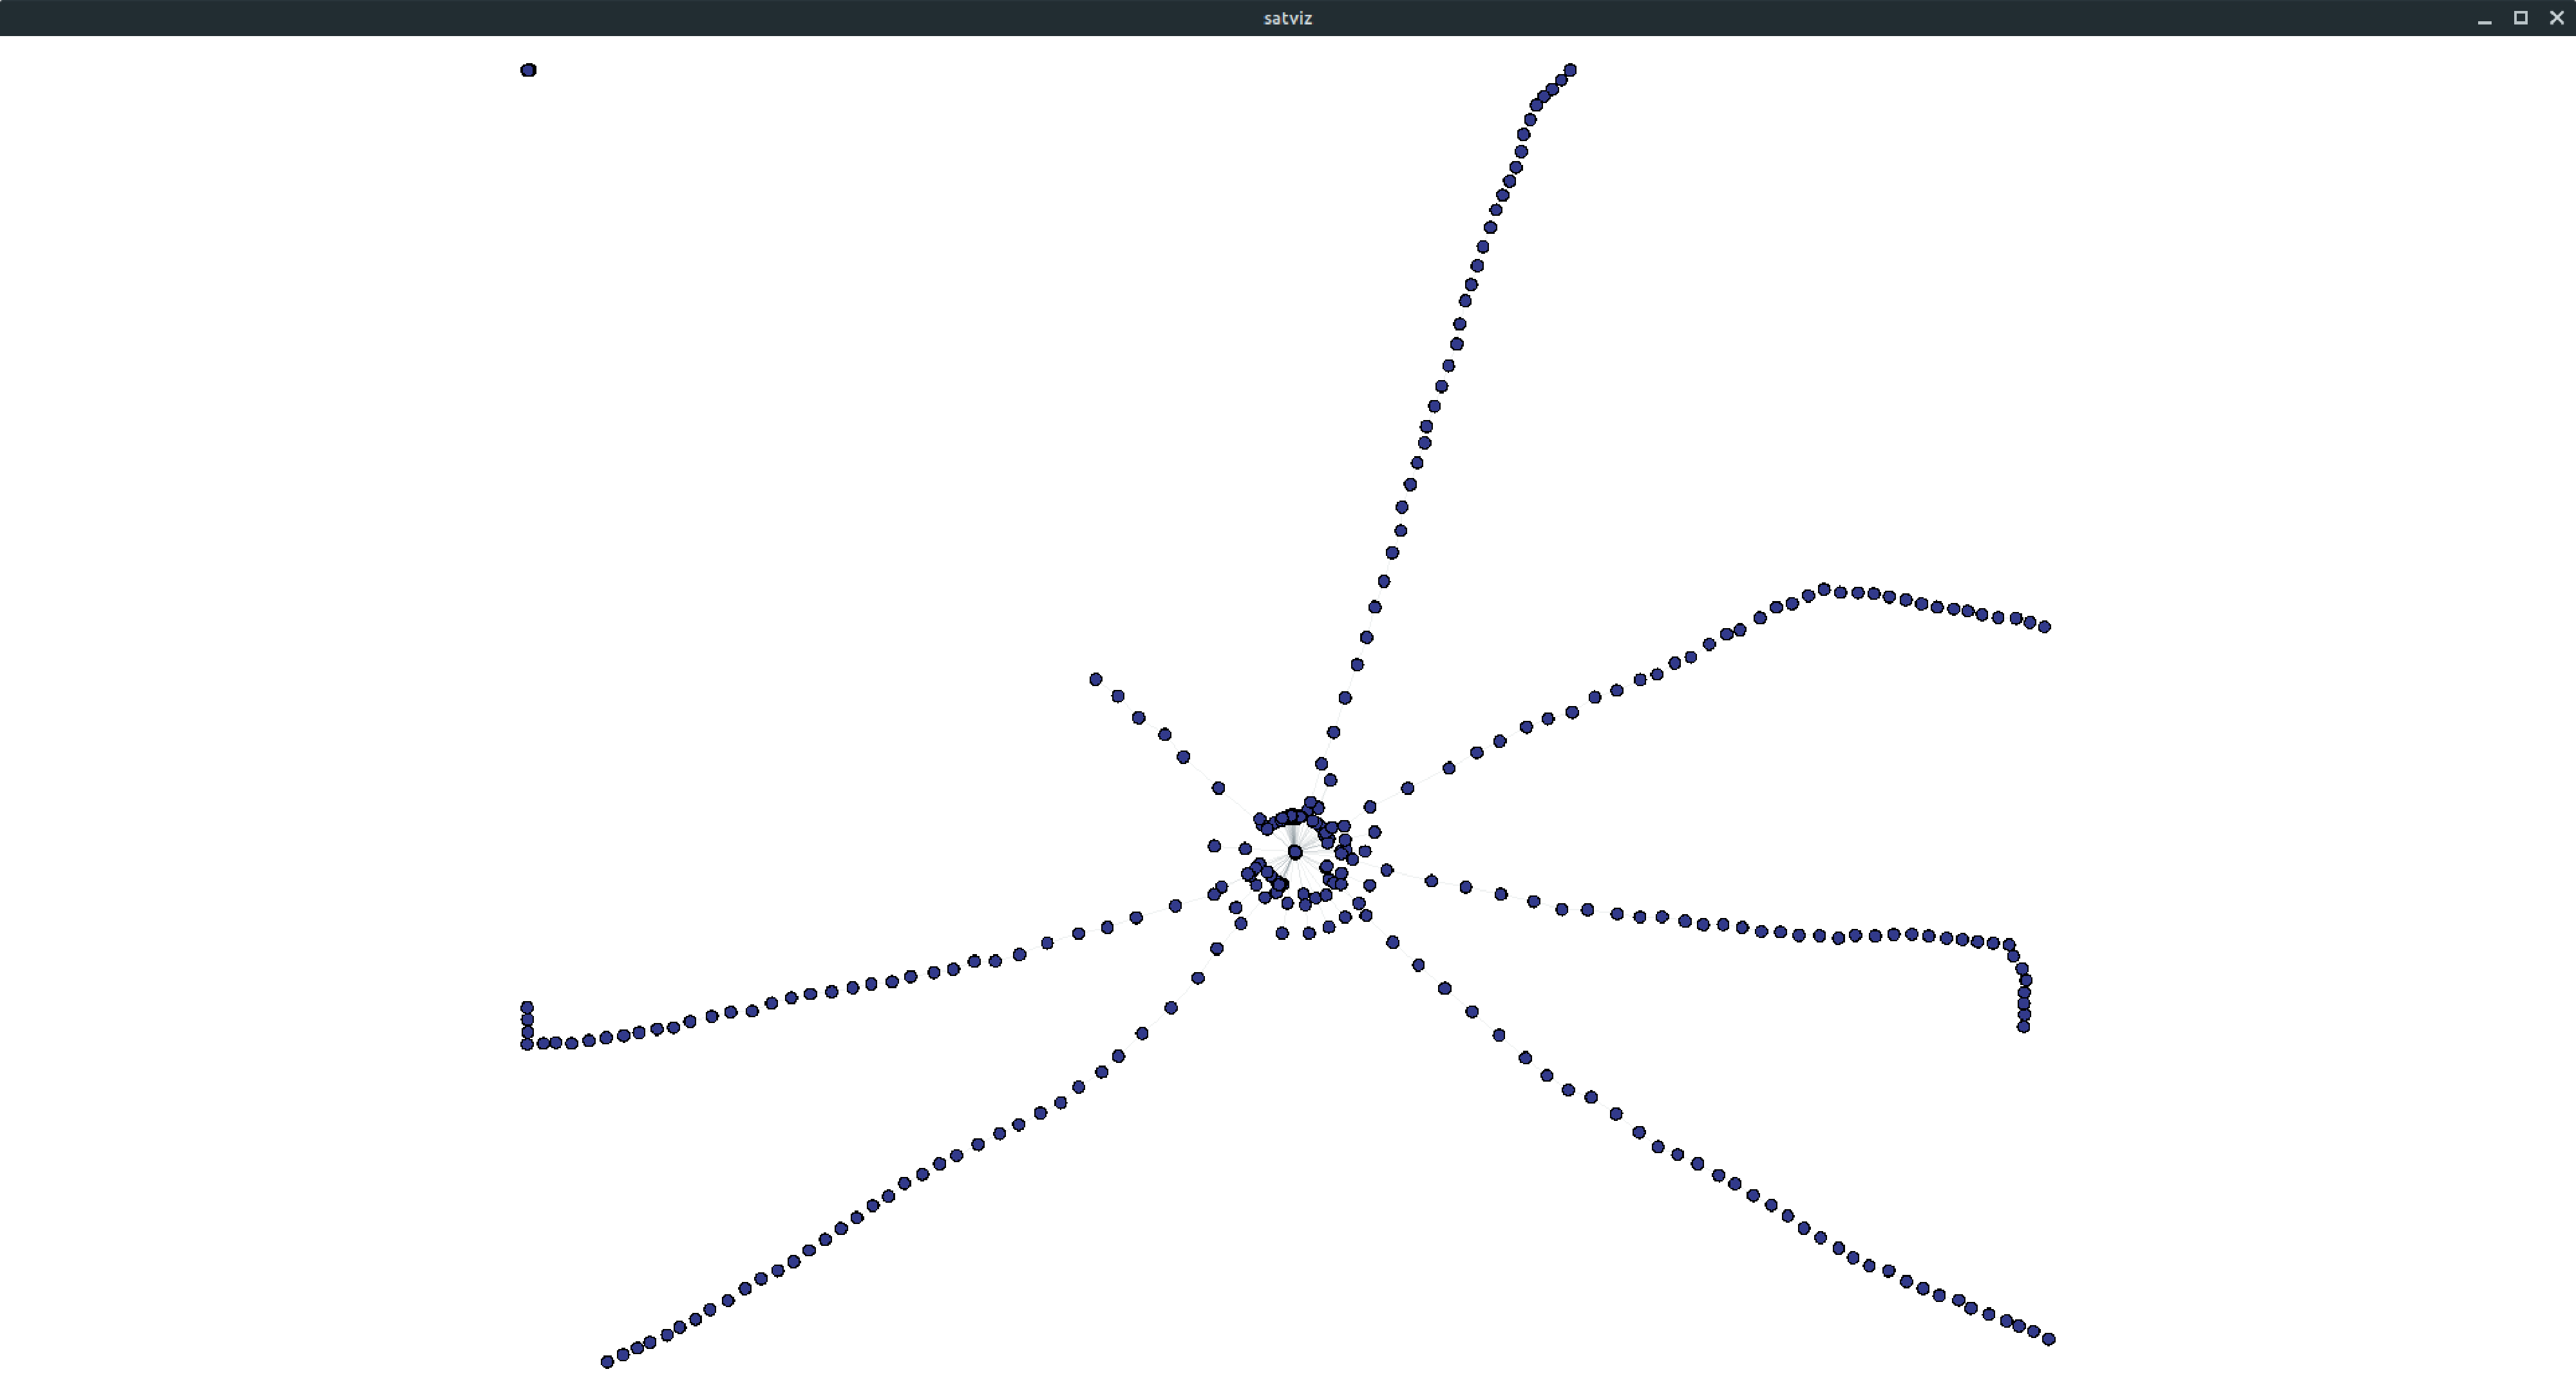
\includegraphics[width=0.9\textwidth, trim={100 0 100 100}, clip]{newton-smt-1000000}
}
\only<4>{
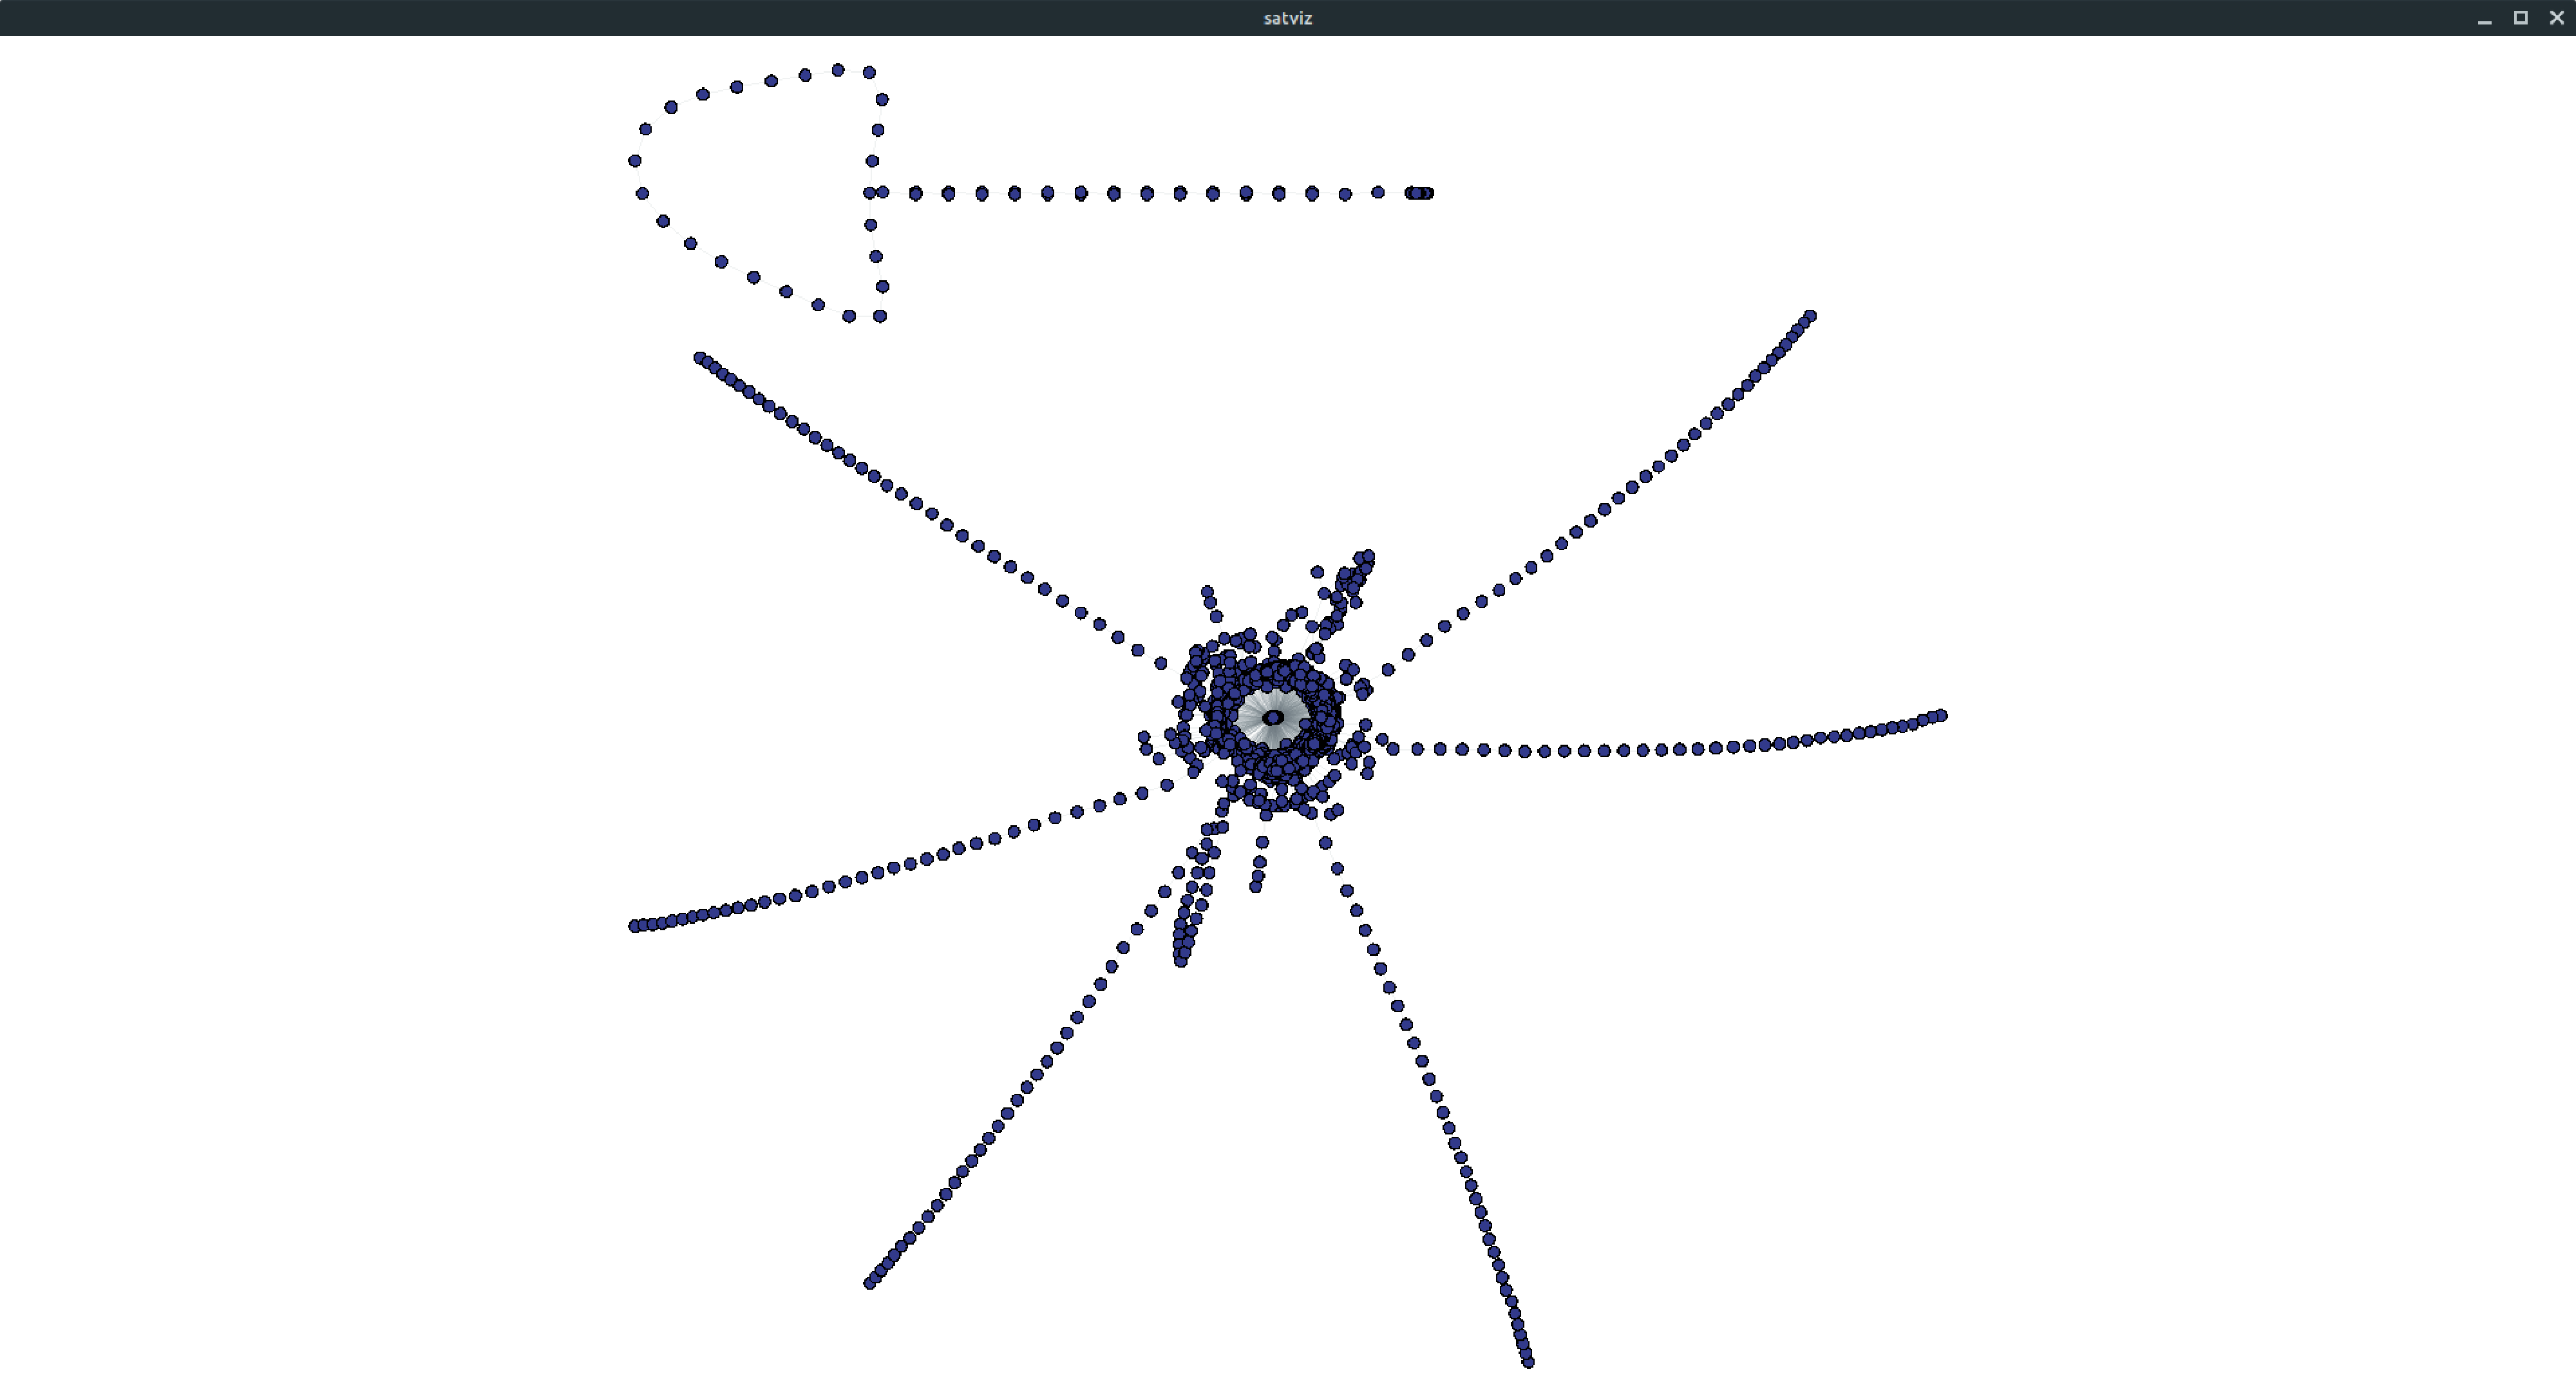
\includegraphics[width=0.9\textwidth, trim={100 0 100 30}, clip]{newton-smt-3000000}
}
\only<5>{
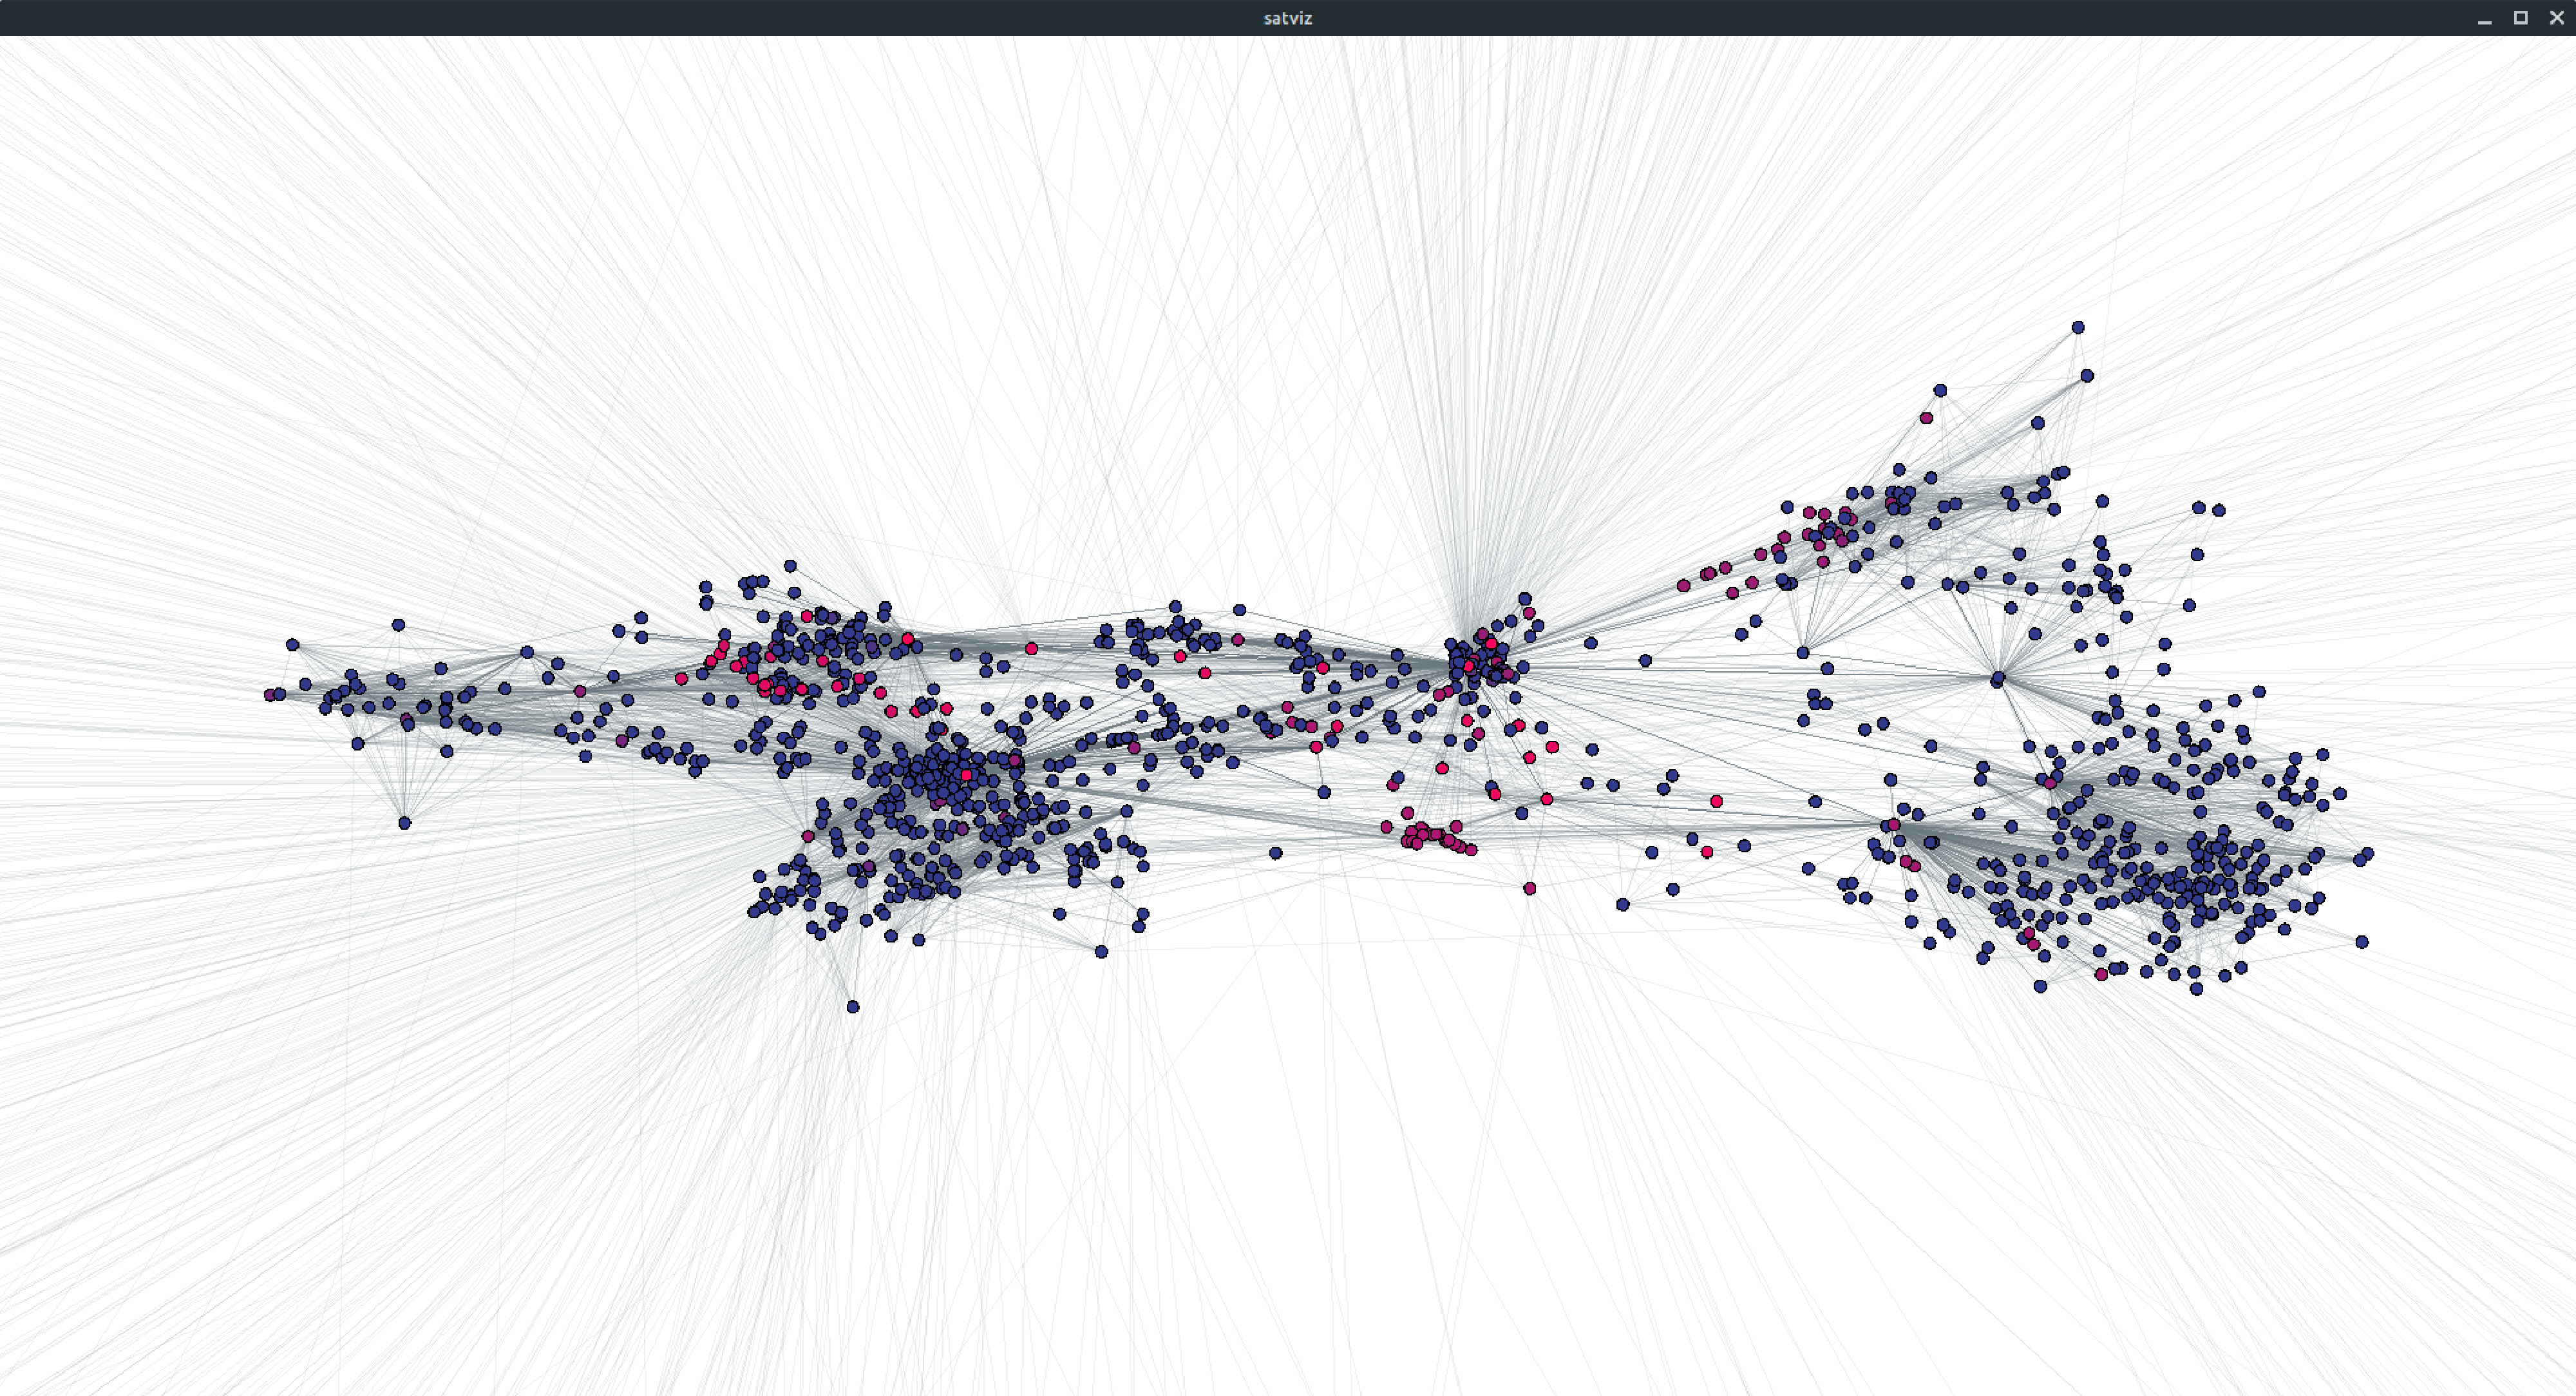
\includegraphics[width=0.9\textwidth, trim={100 0 100 100}, clip]{newton-smt-3500000-cherry}
}
\end{frame}

\begin{frame}{Recap}
\begin{block}{So far}
\begin{itemize}\setlength{\itemsep}{1em}
    \item Efficient Unit Propagation
    \item Clause Forgetting Heuristics:
    \begin{itemize}\setlength{\itemsep}{1ex}
        \item Size, LRU, LBD
        \item Three-Tier Clause Management
    \end{itemize}
\end{itemize}
\end{block}
\begin{block}{Next Up}
Modern Decision Heuristics
\end{block}
\end{frame}

    
\begin{frame}{{\bf V}ariable {\bf S}tate {\bf I}ndependent {\bf D}ecaying {\bf S}um {\bf (VSIDS)}}
\begin{block}{VSIDS Heuristic}
    Implemented in most CDCL solvers. First presented in SAT solver Chaff.\footnote{\href{https://doi.org/10.1145/378239.379017}{Chaff: Engineering an efficient SAT solver (Moskewicz et al., 2001)}}\\[1em]
    Always select variable with highest score for branching. Scores are updated after each conflict.\\[1em]
    \begin{itemize}\setlength{\itemsep}{1em}
        \item Initialize variable score (with zero or use some static heuristic)
        \item New conflict clause $c$: score is incremented for all variables in $c$
        \item Periodically, divide all scores by a constant
    \end{itemize}	
\end{block}
\end{frame}
    
\begin{frame}{{\bf V}ariable {\bf S}tate {\bf I}ndependent {\bf D}ecaying {\bf S}um {\bf (VSIDS)}}
\begin{exampleblock}{Example: Score Update after Conflict}
\begin{columns}[T]
\begin{column}{.45\linewidth}
~\\[1ex]
\textbf{Formula:}
\begin{align*}
    & \{ x_1, x_4 \}, \{ x_1, \overline{x_3}, \overline{x_8} \},  \{ x_1, x_8, x_{12} \}, \{ x_2, x_{11} \}, \\
    & \{ \overline{x_7}, \overline{x_3}, x_9 \}, \{ \overline{x_7}, x_8, \overline{x_9} \}, \{ x_7, x_8, \overline{x_{10}} \}\\
    & {\color{myred} \{ x_7, x_{10}, \overline{x_{12}} \}  \quad } \tag{{\color{myred} new learned clause}}\\
\end{align*}
\end{column}
\begin{column}{.25\linewidth}
~\\[1ex]
\textbf{Scores before:}
\begin{flalign*}
    &4: x_8 &&\\
    &3: x_1, x_7 &&\\
    &2: x_3 &&\\
    &1: x_2, x_4, x_9, x_{10}, x_{11}, x_{12} &&
\end{flalign*}
\end{column}
\begin{column}{.2\linewidth}
~\\[1ex]
\textbf{Scores after:}
\begin{flalign*}
    &4:x_8, {\color{myred} x_7} &&\\
    &3: x_1 &&\\
    &2: x_3, {\color{myred} x_{10}}, {\color{myred} x_{12}} &&\\
    &1: x_2, x_4, x_9, x_{11} &&
\end{flalign*}
\end{column}
\end{columns}
\end{exampleblock}
\pause
\begin{block}{}
\begin{itemize}\setlength{\itemsep}{1ex}
    \item VSIDS leads to more ``focused'' search
    \item prefers variables that occurred in recent conflicts
    \item tends to find smaller unsatisfiable subsets
\end{itemize}
\end{block}
\end{frame}
    
\begin{frame}{{\bf V}ariable {\bf S}tate {\bf I}ndependent {\bf D}ecaying {\bf S}um {\bf (VSIDS)}}
Keep list of variables sorted by scores
\begin{block}{Common implementation: Binary Heap}
    \setcolsep{1em}
    \setrowsep{1.5}
    \begin{tabularx}{\linewidth}{llX}
    \bf Heap Operation & \bf Complexity & \bf Callee\\
    \hline
    \tt insert\_with\_priority & $\mathcal{O}(\log n)$ & Backtracking\\
    \tt pull\_highest\_priority\_element & $\mathcal{O}(\log n)$ & Branching\\
    \tt increase\_key / bump\_variable & $\mathcal{O}(\log n)$ & Conflict Analysis\\
    \tt decay & $\mathcal{O}(n)$ & [Periodic]\footnote{Periodically divide scores to give priority to recently learned clauses}
    \end{tabularx}
\end{block}
\end{frame}
    
\begin{frame}{{\bf V}ariable {\bf S}tate {\bf I}ndependent {\bf D}ecaying {\bf S}um {\bf (VSIDS)}}
\vspace*{-1ex}
\begin{exampleblock}{VSIDS Variants}
\textbf{Chaff (2001)}
\begin{itemize}
    \item decay: half scores every 256 conflicts
    \item sort priority queue after each decay only
\end{itemize}
\textbf{Berkmin (2002)}
\begin{itemize}
    \item bump all literals in implication graph
    \item divide scores by 4
\end{itemize}
\textbf{Minisat (2003)}
\begin{itemize}
    \item Exponential VSIDS (EVSIDS)
    \item Reason-side Bumping
\end{itemize}
\end{exampleblock}
%
\begin{block}{Alternatives}
\textbf{Siege (2004)}: Variable Move To Front (VMTF) \qquad \textbf{HaifaSAT (2008)}: Clause Move To Front (CMTF)
\end{block}
\end{frame}
    
\begin{frame}{\href{https://doi.org/10.1007/978-3-319-24318-4_29}{``Evaluating CDCL Variable Scoring Schemes''}}{\href{https://doi.org/10.1007/978-3-319-24318-4_29}{Biere \& Fröhlich, 2015}}
\vspace*{-3em}
\centering
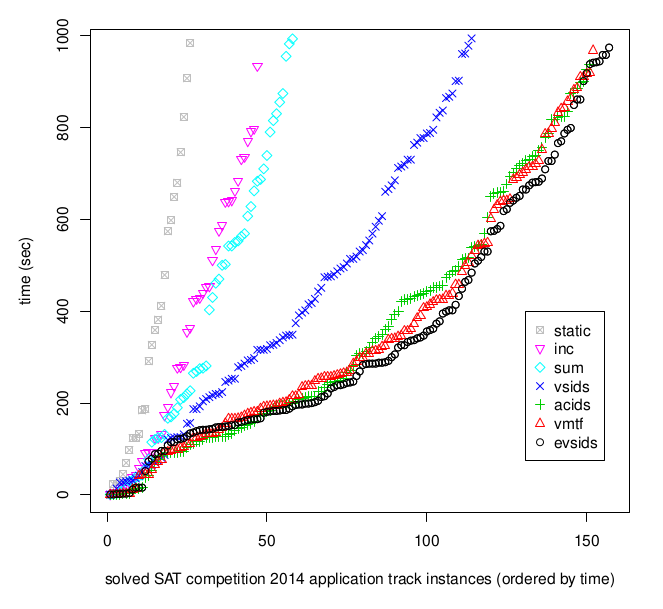
\includegraphics[width=.56\linewidth]{figures/l06/evsids-vmtf-acids-froehlich2015.png}
\end{frame}
    
\begin{frame}{Recent Hybrid Approaches}
\begin{block}{Hybrid Approaches} 
\begin{itemize}\setlength{\itemsep}{1em}
\item {\bf Warmup Phase}:
\begin{itemize}\setlength{\itemsep}{1ex}
    \item MapleCOMSPS (2016): use Learning Rate-based Branching (LRB) in \emph{initial} period, then switch to VSIDS
    \item Maple\_LCM\_Dist (2017): use Distance Heuristic (Dist.) in \emph{initial} period, then switch to VSIDS
\end{itemize}
\item {\bf Reinforcement Learning}: Kissat\_MAB (2021)
\begin{itemize}\setlength{\itemsep}{1ex}
    \item Two-armed Bandid switches between VSIDS and Conflict History-Based (CHB) Heuristic
    \item Reward function favors variables that contribute to learning ``good'' clauses
    \end{itemize}
\end{itemize}
\end{block}
\end{frame}


\begin{frame}{Recap}
    \begin{block}{So far}
        \begin{itemize}
            \item Unit Propagation
            \item Clause Forgetting
            \item Modern Branching Heuristics
            \begin{itemize}
                \item Mostly VSIDS
                \item Hybrid approaches: warmup VSIDS scores, reinforcement learning
            \end{itemize}
        \end{itemize}
    \end{block}
    \begin{block}{Next Up}
        Preprocessing
    \end{block}
\end{frame}
    
\begin{frame}{Preprocessing}
\textbf{Conjecture:} Smaller problems are easier to solve\\[1ex]
$\Longrightarrow$ Try to reduce the size of the input formula by (polynomial time) simplification procedures.\\[1em]
\begin{block}{Today: Basic Preprocessing}
\begin{itemize}\setlength{\itemsep}{1ex}
    \item Subsumption
    \item Self-subsuming Resolution
    \item (Bounded) Variable Elimination (BVE)
    \item Blocked Clause Elimination (BCE)
\end{itemize}
\end{block}
\end{frame}
    
    
\begin{frame}{Subsumption}
A clause $C$ is subsumed by $D$ iff $D \subseteq C$.\\[1ex]
Subsumed clauses can be removed from the formula without changing satisfiability.\\[1ex]
$\forall D \subseteq C, D \models C$\\[1em]
\begin{exampleblock}{Example}
    $\{a, b\}$ subsumes $\{a, b, c\}$ and $\{a, b, d\}$
\end{exampleblock}
\end{frame}
    
    
\begin{frame}{Self-Subsuming Resolution}
Applicable if the resolvent of $C$ and another clause $D$ subsumes $C$.\\[1ex]
Let $C, D$ be clauses and $\otimes_x$ the resolution operator on variable $x$.\\[1ex]
If $C \otimes_x D \subseteq C$ then $C$ can be replaced by $C \otimes_x D$.\\[1em]
   
\begin{exampleblock}{Example}
    $C := \{ \lnot b, \lnot e, {\color{myblue} f}, \lnot h \}$ \qquad
    $D := \{ \lnot b, \lnot e, {\color{myblue} \lnot f} \}$ \qquad
    $E := C \otimes_f D = \{ \lnot b, \lnot e, \lnot h \}$ \\[1em]
    $\bm\longrightarrow$ Replace $C$ by $E$
\end{exampleblock}
\end{frame}
    
    
\begin{frame}{Bounded Variable Elimination (BVE)}
Let $S_x, S_{\overline x} \subset F$ be the sets of all clauses containing $x$ resp. ${\overline x}$, 
and let $R = \{ C \otimes_x D ~|~ C \in S_x, D \in S_{\overline x} \}$ be the set of all resolvents on $x$.\\[1em]
\textbf{Variable Elimination}: Modify $F$ such that \highl{$F' := (F \setminus (S_x \cup S_{\overline x})) \cup R$}\\[1ex]
The formulas $F$ and $F'$ are \highlo{satisfiability equivalent} (why not equivalent?)\\[1em]
%
\textbf{Bounded Variable Elimination}: Eliminate variable only if \highl{size of formula} decreases.\\[1ex]
Most important simplification technique today
\end{frame}
    
    
\begin{frame}{Blocked Clause Elimination (BCE)}
A clause \highl{$\{ l \} \cup C$ is blocked in $F$ by $l$} if 
\begin{itemize}
    \item either $l$ is \emph{pure} in $F$ or
    \item for every clause $\{ \lnot l \} \cup D$ in $F$ the resolvent $C \cup D$ is a \emph{tautology}.
\end{itemize}~\\[1ex]
Removal of an arbitrary blocked clause \highlo{preserves satisfiability}.\\[1ex]
Blocked clause elimination (BCE) has a unique fixpoint.
%
\begin{exampleblock}{Example}
$F := (a \lor b) \land (a \lor \lnot b \lor \lnot c) \land (\lnot a \lor c)$\\[1ex]
First clause is not blocked, second is blocked by both $a$ and $\lnot c$, third is blocked by $c$.
\end{exampleblock}
\end{frame}


\begin{frame}{Recap}
    \begin{block}{Today}
        \begin{itemize}\setlength{\itemsep}{1em}
            \item Unit Propagation
            \item Clause Forgetting
            \item Modern Branching Heuristics
            \item Preprocessing
            \begin{itemize}\setlength{\itemsep}{1ex}
                \item Subsumption
                \item Self-Subsuming Resolution
                \item Bounded Variable Elimination
                \item Blocked Clause Elimination
            \end{itemize}
        \end{itemize}
    \end{block}
\end{frame}


% \begin{frame}{Blocked Clauses and Gates}
% \begin{block}{Left-Totality of Gate Encodings}
%     Given a gate~$G$ with output variable $o$ and its clausal encoding $E$, 
%     it holds that for every clause $C \in E$ either $o \in C$ or $\overline o \in C$ (part~1)
%     and all resolvents in $E[o] \otimes_o E[\overline o]$ are tautologic (part~2).
%     \end{block}
    
%     \begin{block}{Proof of Part 1}
%     Assume that there is a clause $C \in E$ such that $o \not\in \vars{C}$. 
%     It follows that there exists an assignment to input variables which falsifies $C$ for any assignment to $o$. 
%     This contradicts left-totality.
%     \end{block}
    
%     \begin{block}{Proof of Part 2}
%     Let $R$ be a non-tautological resolvent in $E[o] \otimes_o E[\overline o]$. 
%     By Definition of resolution, it holds that $o \not\in \vars{R}$ and $E \models R$. 
%     This contradicts left-totality. 
% \end{block}
% \end{frame}
    
    
% \begin{frame}{Variable Elimination and Gates}
% \begin{block}{Property of Gate Encodings}
%     \begin{itemize}
%     \item Resolving the clauses of a gate results in tautological clauses
%     \item Example: Tseitin encoding of gate $x = \mathop{AND}(y,z)$ results in the clauses $\{ \lnot x, y \}, \{ \lnot x, z \}, \{ x, \lnot y, \lnot z \}$
%     \end{itemize}
% \end{block}

% \begin{block}{Idea: Variable Elimination for Gate Encoding $G$}
%     \begin{itemize}
%     \item Split formula $F$ into $F = G \cup R$, where $G$ are the gate clauses
%     \item Apply variable elimination:\vspace*{-.7em}
%     \begin{align*}
%     S' &= (G_x \cup R_x) \otimes (G_{\overline x} \cup R_{\overline x})\\
%        &= (G_x \otimes R_{\overline x}) \cup (R_x \otimes G_{\overline x}) \cup (R_x \otimes R_{\overline x}) \cup \hcancel{(G_x \otimes G_{\overline x})}\\
%        &= (G_x \otimes R_{\overline x}) \cup (R_x \otimes G_{\overline x}) \cup \hcancel{(R_x \otimes R_{\overline x})}\\
%        &= (R_x \otimes G_{\overline x}) \cup (R_{\overline x} \otimes G_x)
%     \end{align*}\vspace*{-2em}%
%     \item $(G_x \otimes R_{\overline x}) \cup (R_x \otimes G_{\overline x}) \models (R_x \otimes R_{\overline x})$ {\color{mypink} (Why? $\rightarrow Exercise$)}
%     \end{itemize}
% \end{block}
% \end{frame}
    

% \begin{frame}{Failed Literal Elimination}
% \begin{block}{Definition}
% If $F \land \{ l \} \vdash_{\mathop{UP}} \bot$, i.e., applying unit propagation on $F \land \{ l \}$ derives UNSAT, replace $F$ by $F \land \{ \lnot l\}$.
% \end{block}
    
% \begin{block}{Generalization} 
% If $(F \setminus \{ C \}) \land \lnot C \vdash_{\mathop{UP}} \bot$, remove $C$ from $F$.
% \end{block}
% \end{frame}

    
% \begin{frame}{Autarkies}
% \begin{block}{Definition}
% Given a partial assignment $\sigma$ and a formula $F$, a clause $C \in F$ is \emph{touched by $\sigma$} if it contains the negation of a literal 
% assigned in $\sigma$. A clause  is \emph{satisfied by $\sigma$} if it contains a literal assigned to $\true$ by $\sigma$.
% If all touched clauses are satisfied then $\sigma$ is an \emph{autarky}.
% \end{block}

% All clauses touched by an autarky can be removed.

% \begin{exampleblock}{Autarky-based Clause Removal}
% The partial assignment $\sigma = \{ \lnot a, \lnot c \}$ is an autarky for $F := \{ \lnot a, b \}, \{ \lnot a, c \}, \{ a, \lnot b, \lnot c \}, \{ b, d \}, \dots$ (more clauses without $a$ and $c$)
% \end{exampleblock}
% \end{frame}
    
    
% \begin{frame}{Preprocessing Techniques that do not Reduce the Problem Size}
% \begin{itemize}
% \item Bounded Variable Addition (BVA) a.k.a. Extension rule
% \item Some formulas have refutations of exponential size in the resolution calculus, but of polynomial size in extended resolution, e.g., pigeonhole formulas, mutilated chessboard, \dots
% \end{itemize}
% \begin{block}{Extended Resolution}
% Extended resolution adds a second rule to the resolution calculus, the Extension Rule. The idea is to introduce
% new variables as conjunction of existing literals, $x_\mathrm{new} \leftrightarrow l_1 \land l_2$. As a rule for formulas in CNF:
% \vspace{-2ex}
% $$ \cfrac{}{(\lnot x_\mathrm{new} \lor l_1) \land (\lnot x_\mathrm{new} \lor l_2) \land (x_\mathrm{new} \lor \lnot l_1 \lor \lnot l_ 2) } $$
% \end{block}
% \end{frame}
    

% \begin{frame}{Inprocessing}

% \begin{block}{Idea: Interleave search and preprocessing}
% \begin{itemize}
% \item Preprocessing can be extremely beneficial
% \item Most solvers in SAT competitions use bounded variable elimination, subsumption and self-subsuming resolution
% \item Problem: Many preprocessing techniques, though polynomial, require considerable time
% \item Possible Solutions:
% \begin{itemize}
% \item Interrupt preprocessing techniques after some time
% \item Resume preprocessing between restarts
% \item Limit preprocessing time in relation to search
% \end{itemize}
% \end{itemize}
% \end{block}
% \end{frame}


% \begin{frame}{Hybrid Backtracking}
%     \begin{block}{Recent Revival of Chronological Backtracking}
%     \begin{itemize}
%     \item Nadel \& Ryvchin, SAT 2018
%     \item Backtrack chronologically iff number of untouched decision levels is higher than a given bound
%     \item SAT Competition 2018: \texttt{MapleLCMDistChronoBT} (best score)
%     \item SAT Race 2019: \texttt{MapleLCMDistChronoBT} \& \texttt{CaDiCal} (best scores)
%     \item Hard to implement: Decision levels no longer monotonically increasing on trail
%     \end{itemize}
%     \end{block}
% \end{frame}

\end{document}
